\documentclass[12pt,a4paper]{report}

\usepackage{iftex}
\ifXeTeX
    \usepackage{fontspec}
    \setmainfont{Times New Roman}
    \usepackage{polyglossia}
    \setdefaultlanguage{vietnamese}
\else
    \usepackage[utf8]{inputenc}
    \usepackage[vietnamese]{babel}
    \usepackage{times}
\fi

\usepackage{graphicx}
\usepackage{tikz}
\usetikzlibrary{calc, arrows.meta, positioning, shapes.geometric, trees}
\usepackage{enumitem}
\usepackage{listings}
\usepackage{longtable}
\usepackage{amsmath}
\usepackage{fancyvrb}
\usepackage{indentfirst}
\usepackage{multirow}
\usepackage{tocloft}
\usepackage{array}
\usepackage{makecell}
\usepackage{ragged2e}
\usepackage{colortbl}
\usepackage{titlesec}
\usepackage{caption}
\usepackage{tabularx}
\usepackage{float}

% Định nghĩa màu sắc in ấn học thuật (100% Black)
\definecolor{kiotblue}{RGB}{0, 0, 0}
\definecolor{kiotdark}{RGB}{0, 0, 0}
\definecolor{kiotgreen}{RGB}{0, 0, 0}
\definecolor{kiotgray}{RGB}{80, 80, 80}
\definecolor{tableheader}{gray}{0.90}

% Định dạng tiêu đề chương mục chuẩn đồ án
\titleformat{\chapter}[hang]
  {\normalfont\LARGE\bfseries}{\chaptertitlename\ \thechapter:}{0.5em}{}
\titlespacing*{\chapter}{0pt}{-10pt}{20pt}

\titleformat{\section}
  {\normalfont\Large\bfseries}{\thesection}{1em}{}
\titlespacing*{\section}{0pt}{15pt}{8pt}

\titleformat{\subsection}
  {\normalfont\large\bfseries}{\thesubsection}{1em}{}
\titlespacing*{\subsection}{0pt}{12pt}{6pt}

\titleformat{\subsubsection}
  {\normalfont\normalsize\bfseries}{\thesubsubsection}{1em}{}
\titlespacing*{\subsubsection}{0pt}{8pt}{4pt}

% Giãn dòng 1.3 và thụt đầu dòng 1cm
\renewcommand{\baselinestretch}{1.3}
\setlength{\parindent}{1cm}
\setlength{\parskip}{4pt}

% Cấu hình hiển thị mã nguồn
\lstdefinestyle{csharp}{
    backgroundcolor=\color{gray!5},
    basicstyle=\ttfamily\footnotesize\color{black},
    keywordstyle=\bfseries\color{black},
    commentstyle=\itshape\color{gray!70},
    stringstyle=\color{black},
    breaklines=true,
    breakatwhitespace=true,
    tabsize=2,
    showstringspaces=false,
    numbers=left,
    numberstyle=\tiny\color{gray},
    frame=single,
    rulecolor=\color{gray!40},
    captionpos=b
}
\lstset{style=csharp}

% Cấu hình cột bảng
\makeatletter
\newcommand{\thickhline}{%
    \noalign {\ifnum 0=`}\fi \hrule height 1pt
    \futurelet \reserved@a \@xhline
}
\newcolumntype{Y}{>{\raggedright\arraybackslash}X}
\makeatother

% Căn lề chuẩn đồ án A4
\usepackage{geometry}
\geometry{left=3cm, right=2cm, top=2.5cm, bottom=2.5cm}

\usepackage{hyperref}
\hypersetup{
    colorlinks=true,
    linkcolor=black,
    filecolor=black,      
    urlcolor=black,
    citecolor=black,
    pdftitle={Bao Cao Bai Tap Lon - Website Quan Ly Kho Hang Da Chi Nhanh},
    pdfauthor={Nhom 3 - DH GTVT},
    bookmarksopen=true
}

\begin{document}

% ==========================================
% TRANG BÌA CHUẨN ĐH GIAO THÔNG VẬN TẢI (KHÔNG VIỀN)
% ==========================================
\begin{titlepage}
    \begin{center}
        {\Large \textbf{TRƯỜNG ĐẠI HỌC GIAO THÔNG VẬN TẢI}}\\[0.2cm]
        {\Large \textbf{KHOA CÔNG NGHỆ THÔNG TIN}}\\[0.5cm]
        
        % Logo Trường ĐH Giao thông Vận tải
        \IfFileExists{GTVT1.jpg}{%
            
\includegraphics[width=4.2cm]{GTVT1.jpg}\\[0.4cm]
        }{%
            
\includegraphics[width=4.2cm]{logo_gtvt.jpg}\\[0.4cm]
        }

        {\Huge \textbf{BÀI TẬP LỚN}}\\[0.35cm]
        {\Large \textbf{Môn học : Lập trình Web}}\\[0.45cm]
        {\LARGE \textbf{Đề tài : Xây Dựng Website Quản Lý Kho Hàng\\[0.35cm] Đa Chi Nhánh}}\\[0.6cm]
        
        % Thông tin sinh viên và giảng viên
        \renewcommand{\arraystretch}{1.25}
        \begin{tabular}{@{}ll@{}}
            \textbf{Giảng viên hướng dẫn} & : Đào Thị Lệ Thủy \\[0.12cm]
            \textbf{Khoa}                 & : Công nghệ thông tin \\[0.12cm]
            \textbf{Nhóm thực hiện}       & : Nhóm 3 -- Lớp N04 -- K65 \\[0.12cm]
            \textbf{Sinh viên thực hiện}  & : Bùi Tuấn Anh -- 241230653 (Trưởng nhóm)\\[0.12cm]
                                          & : Phạm Văn Hào -- 241224475 \\[0.12cm]
                                          & : Nguyễn Minh Khuê -- 231230815 \\[0.12cm]
                                          & : Nguyễn Thị Tuyết Mai -- 241230783 \\[0.12cm]
        \end{tabular}
        
        \vfill
        
        {\large \textbf{Hà Nội, tháng 9 năm 2026}}
    \end{center}
\end{titlepage}

% ==========================================
% TRANG LỜI NÓI ĐẦU
% ==========================================
\clearpage
\begin{center}
    \vspace*{0.5cm}
    {\Huge \textbf{Lời nói đầu}}
    \vspace{0.5cm}
\end{center}

Trong bối cảnh cuộc Cách mạng công nghiệp lần thứ tư và công cuộc chuyển đổi số đang diễn ra mạnh mẽ tại Việt Nam, việc ứng dụng công nghệ thông tin vào quản trị doanh nghiệp, đặc biệt là công tác quản lý kho bãi và chuỗi cung ứng, đóng vai trò sống còn đối với sự phát triển bền vững của mỗi tổ chức. Đối với các doanh nghiệp sở hữu từ hai chi nhánh kho trở lên, bài toán quản lý kho càng trở nên nan giải do tình trạng thất thoát hàng hóa, sai lệch tồn kho giữa sổ sách và thực tế, khó khăn trong việc điều chuyển hàng hóa liên chi nhánh và thiếu đi góc nhìn tổng quan theo thời gian thực. Một hệ thống thông tin quản lý kho chuyên nghiệp được xây dựng trên nền tảng web không chỉ giúp loại bỏ hoàn toàn các thao tác thủ công dễ sai sót mà còn hỗ trợ nhân viên tra cứu tức thì, hạn chế tối đa rủi ro tài chính và nâng cao năng lực cạnh tranh trong vận hành.

Trong thực tế, hoạt động quản trị kho đòi hỏi sự liên kết chặt chẽ giữa nhiều khâu nghiệp vụ khép kín: từ khâu tiếp nhận hàng từ nhà cung cấp, kiểm đếm nhập kho, lưu trữ, điều chuyển nội bộ giữa các kho, xuất hủy hàng hóa hư hỏng/hết hạn sử dụng, cho đến định kỳ kiểm kê và cân bằng sai lệch kho. Mỗi khâu đều phát sinh chứng từ kế toán và yêu cầu sự phối hợp nhịp nhàng giữa ba lớp nhân sự: Quản trị viên, Thủ kho và Nhân viên kho. Nếu các chứng từ và số lượng biến động không được quản lý tập trung và bọc trong các giao dịch an toàn (ACID Transaction), việc thất thoát và xác định trách nhiệm khi xảy ra chênh lệch sẽ trở nên vô cùng phức tạp.

Xuất phát từ những vấn đề thực tiễn trên, nhóm sinh viên lựa chọn đề tài \textbf{``Xây Dựng Website Quản Lý Kho Hàng Đa Chi Nhánh''} làm nội dung nghiên cứu cho bài tập lớn học phần \textbf{Lập trình Web}. Đề tài tập trung nghiên cứu, phân tích nghiệp vụ thực tế và hiện thực hóa một hệ sinh thái quản lý kho chuyên nghiệp trên nền tảng công nghệ tiên tiến nhất \textbf{ASP.NET Core MVC (.NET 10)}, Entity Framework Core 10 và hệ quản trị cơ sở dữ liệu Microsoft SQL Server, mô phỏng chuẩn mực theo trải nghiệm và quy trình vận hành ưu việt của phần mềm KiotViet.

Hệ thống được thiết kế phục vụ người dùng nội bộ, giải quyết triệt để bài toán đồng bộ tồn kho bằng giải thuật tính toán động qua Database View (\texttt{vw\_TonKhoHienTai}, \texttt{vw\_BienDongKho}), đóng gói hệ sinh thái giao diện khối Lego UI tái sử dụng và cung cấp các báo cáo phân tích chuyên sâu (Báo cáo Tồn kho đa chi nhánh dạng Pivot và Báo cáo Thẻ kho tịnh tiến lũy kế).

Báo cáo trình bày đầy đủ quá trình từ khảo sát hiện trạng, phân tích yêu cầu nghiệp vụ, thiết kế biểu đồ Use Case, thiết kế cơ sở dữ liệu quan hệ ERD, sitemap, wireframe giao diện, chi tiết quá trình lập trình triển khai hệ thống, danh mục kiểm thử test cases thực tế và đánh giá kết quả đạt được. Thông qua đề tài, nhóm có cơ hội vận dụng sâu sắc kiến thức được học trong học phần Lập trình Web vào một bài toán thực tiễn có độ phức tạp cao, đồng thời rèn luyện kỹ năng làm việc nhóm và giải quyết sự cố kỹ thuật.

Nhóm xin chân thành cảm ơn cô Đào Thị Lệ Thủy cùng các thầy cô trong Khoa Công nghệ Thông tin -- Trường Đại học Giao thông Vận tải đã tận tình giảng dạy, định hướng kiến trúc và góp ý quý báu trong suốt quá trình nhóm thực hiện đề tài. Do kiến thức và thời gian thực hiện còn hạn chế, báo cáo khó tránh khỏi những thiếu sót nhất định. Nhóm rất mong nhận được ý kiến đóng góp của quý thầy cô để hệ thống ngày càng hoàn thiện hơn.

\begin{flushright}
    \textit{Nhóm 3 -- Lớp N04 -- K65}\\
    \textit{Khoa Công nghệ Thông tin -- Trường ĐH Giao thông Vận tải}
\end{flushright}

\cleardoublepage

% ==========================================
% BẢNG PHÂN CÔNG CÔNG VIỆC
% ==========================================
\section*{Bảng phân công công việc}
\addcontentsline{toc}{chapter}{Bảng phân công công việc}

\begin{table}[H]
\centering
\small
\renewcommand{\arraystretch}{2.0}
\begin{tabularx}{\linewidth}{|>{\centering\arraybackslash}p{0.8cm}|>{\RaggedRight}p{3.2cm}|>{\centering\arraybackslash}p{2.2cm}|>{\RaggedRight}X|>{\centering\arraybackslash}p{2cm}|>{\centering\arraybackslash}p{1.8cm}|}
\hline
\rowcolor{tableheader}
\textbf{STT} & \textbf{Họ và tên} & \textbf{Vai trò} & \textbf{Nhiệm vụ phân công} & \textbf{Tiến độ} & \textbf{Đánh giá} \\
\hline
1 & \textbf{Bùi Tuấn Anh} & Trưởng nhóm & & & \\
\hline
2 & \textbf{Phạm Văn Hào} & Thành viên & & & \\
\hline
3 & \textbf{Nguyễn Minh Khuê} & Thành viên & & & \\
\hline
4 & \textbf{Nguyễn Thị Tuyết Mai} & Thành viên & & & \\
\hline
\end{tabularx}
\label{tab:phan_cong_cong_viec}
\end{table}

\cleardoublepage

% ==========================================
% DANH MỤC THUẬT NGỮ VÀ TỪ VIẾT TẮT
% ==========================================
\section*{Danh mục thuật ngữ và từ viết tắt}
\addcontentsline{toc}{chapter}{Danh mục thuật ngữ và từ viết tắt}

\begin{table}[H]
\centering
\small
\renewcommand{\arraystretch}{1.3}
\begin{tabularx}{\textwidth}{|>{\bfseries}p{2.5cm}|p{4.5cm}|Y|}
\hline
\rowcolor{tableheader}
Từ viết tắt & Thuật ngữ tiếng Anh & Ý nghĩa / Giải thích trong đề tài \\
\hline
ASP.NET Core & Active Server Pages .NET Core & Khung ứng dụng web mã nguồn mở, đa nền tảng, hiệu năng cao của Microsoft \\
\hline
MVC & Model -- View -- Controller & Kiến trúc phần mềm tách biệt Dữ liệu (Model), Giao diện (View) và Điều khiển (Controller) \\
\hline
EF Core & Entity Framework Core & Bộ ánh xạ đối tượng -- quan hệ (ORM) cho .NET, hỗ trợ tương tác CSDL qua mã C\# \\
\hline
SQL & Structured Query Language & Ngôn ngữ truy vấn có cấu trúc dùng để quản lý cơ sở dữ liệu quan hệ \\
\hline
DBMS & Database Management System & Hệ quản trị cơ sở dữ liệu (trong đề tài sử dụng Microsoft SQL Server) \\
\hline
ACID & Atomicity, Consistency, Isolation, Durability & 4 thuộc tính đảm bảo tính toàn vẹn và tin cậy của giao dịch cơ sở dữ liệu \\
\hline
AJAX & Asynchronous JavaScript and XML & Kỹ thuật tải và gửi dữ liệu không đồng bộ, giúp cập nhật trang web không cần tải lại \\
\hline
JSON & JavaScript Object Notation & Định dạng trao đổi dữ liệu nhẹ dạng văn bản giữa Web Browser và Web API Controller \\
\hline
REST API & REpresentational State Transfer API & Chuẩn giao tiếp lập trình ứng dụng qua các phương thức HTTP (GET, POST...) \\
\hline
UI / UX & User Interface / User Experience & Giao diện người dùng và Trải nghiệm người dùng \\
\hline
SKU & Stock Keeping Unit & Mã định danh duy nhất của từng mặt hàng nội bộ (ví dụ: HH0001, SP002) \\
\hline
DVT & Đơn vị tính & Đơn vị đo lường cơ sở của hàng hóa (ví dụ: Thùng, Hộp, Chai, Cái, Kg) \\
\hline
NCC & Nhà cung cấp & Đối tác cung ứng hàng hóa cho doanh nghiệp \\
\hline
FIFO & First In, First Out & Phương pháp nhập trước xuất trước trong luân chuyển hàng tồn kho \\
\hline
\end{tabularx}
\label{tab:danh_muc_viet_tat}
\end{table}

\cleardoublepage

% ==========================================
% MỤC LỤC TỰ ĐỘNG
% ==========================================
\tableofcontents
\cleardoublepage

% DANH SÁCH HÌNH VẼ
\listoffigures
\addcontentsline{toc}{chapter}{Danh mục hình vẽ}
\cleardoublepage

% DANH SÁCH BẢNG BIỂU
\listoftables
\addcontentsline{toc}{chapter}{Danh mục bảng biểu}
\cleardoublepage

% ==========================================
% CHƯƠNG 1: TỔNG QUAN VÀ PHÂN TÍCH YÊU CẦU BÀI TOÁN
% ==========================================
\chapter{TỔNG QUAN VÀ PHÂN TÍCH YÊU CẦU BÀI TOÁN}

\section{Bối cảnh thực tiễn và lý do chọn đề tài}

\subsection{Thực trạng quản lý lưu chuyển hàng hóa tại các chuỗi chi nhánh kho}
Trong nền kinh tế thị trường cạnh tranh khốc liệt ngày nay, quy mô của các doanh nghiệp bán lẻ và phân phối có xu hướng mở rộng nhanh chóng từ một cửa hàng đơn lẻ thành chuỗi nhiều chi nhánh kho bãi đặt tại các vị trí địa lý khác nhau. Sự gia tăng về số lượng điểm lưu kho mang lại lợi thế tiếp cận khách hàng nhanh chóng nhưng đồng thời đặt ra thách thức quản trị vô cùng lớn:
\begin{itemize}
    \item Hàng hóa luân chuyển liên tục giữa các kho đòi hỏi việc theo dõi nguồn gốc và trạng thái chứng từ phải diễn ra tức thời theo thời gian thực.
    \item Mỗi chi nhánh có tốc độ tiêu thụ khác nhau, dẫn đến tình trạng kho này thừa hàng tồn đọng gây ứ đọng vốn trong khi kho khác lại thiếu hụt hàng hóa dẫn đến mất cơ hội bán hàng.
    \item Đòi hỏi ban lãnh đạo phải có cái nhìn bao quát về tổng tài sản hàng tồn kho trên toàn chuỗi cũng như chi tiết tại từng điểm kho để ra quyết định điều chuyển kịp thời.
\end{itemize}

\subsection{Những bất cập của phương pháp quản lý thủ công và yêu cầu chuyển đổi số}
Thực tế tại nhiều doanh nghiệp vừa và nhỏ cho thấy, công tác quản lý kho vẫn đang phụ thuộc vào sổ sách ghi chép tay hoặc các tệp tin Microsoft Excel dùng chung. Phương pháp truyền thống này bộc lộ hàng loạt rủi ro nghiêm trọng:
\begin{itemize}
    \item \textbf{Sai lệch số liệu và xung đột dữ liệu (Race Conditions):} Khi nhiều thủ kho cùng nhập xuất trên một file Excel chia sẻ qua mạng nội bộ, hiện tượng ghi đè tệp tin xảy ra thường xuyên, làm mất dấu số liệu tồn kho thực tế.
    \item \textbf{Thất thoát hàng hóa và thiếu cơ chế lưu vết (Audit Trail):} Sổ sách thủ công không thể ghi nhận chính xác ai là người tạo phiếu, duyệt xuất kho hay chỉnh sửa số lượng vào thời điểm nào, gây khó khăn khi quy trách nhiệm vật chất.
    \item \textbf{Thời gian kiểm kê kéo dài:} Mỗi đợt kiểm kê định kỳ thường đòi hỏi doanh nghiệp phải dừng hoạt động bán hàng trong nhiều ngày để đếm thủ công, sau đó đối chiếu phức tạp với sổ sách kế toán.
    \item \textbf{Chậm trễ trong báo cáo phân tích:} Việc tổng hợp số liệu tồn kho từ các chi nhánh đòi hỏi hàng giờ làm việc thủ công, không đáp ứng được yêu cầu ra quyết định nhanh của nhà quản trị.
\end{itemize}
Do đó, việc xây dựng một hệ thống website quản lý kho tập trung, hoạt động trên nền tảng đám mây, cho phép truy cập linh hoạt từ mọi thiết bị với độ bảo mật cao là yêu cầu cấp thiết.

\subsection{Mô hình tham chiếu thực tế: Triết lý vận hành phần mềm quản trị KiotViet}
Để đảm bảo sản phẩm phần mềm mang tính ứng dụng cao và phù hợp với thói quen của người dùng Việt Nam, nhóm nghiên cứu đã lựa chọn phần mềm **KiotViet** làm mô hình tham chiếu thực tế. KiotViet hiện là giải pháp quản lý bán hàng và kho phổ biến nhất tại thị trường Việt Nam với các ưu điểm vượt trội:
\begin{itemize}
    \item \textbf{Bố cục 2 cột trực quan:} Cột trái dành riêng cho các bộ lọc thông minh (Lọc theo dải ngày, trạng thái, nhóm hàng, chi nhánh), cột phải là vùng làm việc hiển thị danh sách chứng từ và thanh công cụ tác vụ.
    \item \textbf{Hỗ trợ thao tác phím tắt tối đa:} Tích hợp các phím tắt nhanh (F1 để tra cứu hướng dẫn, F3 để tìm kiếm hàng hóa, F4 để thu gọn thanh lọc, Esc để đóng cửa sổ bật lên) giúp nhân viên kho xử lý nhanh chóng mà không cần lạm dụng chuột.
    \item \textbf{Nguyên tắc bất biến của chứng từ:} Khi một giao dịch kho đã hoàn tất và sinh phiếu kế toán, hệ thống khóa vĩnh viễn quyền chỉnh sửa nhằm đảm bảo tính toàn vẹn và minh bạch của dữ liệu kiểm toán.
\end{itemize}

\section{Phân tích các nghiệp vụ kho cốt lõi}

\subsection{Quản lý danh mục hàng hóa, nhóm hàng và phân cấp đơn vị tính}
Hệ thống cho phép quản trị toàn diện thông tin hàng hóa bao gồm: Mã định danh nội bộ (SKU), Mã vạch quét nhanh (Barcode), Tên sản phẩm, Nhóm hàng phân cấp, Giá vốn bình quân, Giá bán niêm yết, Vị trí kệ lưu trữ và Hình ảnh minh họa. Đặc biệt, hệ thống hỗ trợ thiết lập định mức tồn an toàn (Tồn tối thiểu và Tồn tối đa) để tự động phát tín hiệu cảnh báo khi lượng hàng chạm ngưỡng nguy hiểm.

\subsection{Nghiệp vụ Nhập kho từ Nhà cung cấp và tính toán giá vốn}
Khi tiếp nhận lô hàng từ đối tác cung ứng, thủ kho lập Phiếu Nhập hàng, chọn Nhà cung cấp, quét mã vạch mặt hàng, ghi nhận số lượng và đơn giá nhập thực tế. Hệ thống tự động tính toán tổng tiền hàng, thuế GTGT và tự động cập nhật lại Giá vốn của sản phẩm theo phương pháp bình quân gia quyền tức thời:
\begin{equation}
\text{Giá vốn mới} = \frac{(\text{Tồn hiện tại} \times \text{Giá vốn cũ}) + (\text{Số lượng nhập} \times \text{Đơn giá nhập})}{\text{Tồn hiện tại} + \text{Số lượng nhập}}
\end{equation}
Đồng thời, số lượng tồn kho tại chi nhánh tiếp nhận được cộng tăng ngay lập tức.

\subsection{Nghiệp vụ Trả hàng nhà cung cấp và Nghiệp vụ Xuất hủy hàng hỏng/hết hạn}
\begin{itemize}
    \item \textbf{Trả hàng nhà cung cấp:} Trong trường hợp hàng hóa giao không đúng chất lượng hoặc bị lỗi từ phía đối tác, thủ kho lập Phiếu Trả hàng nhập, hệ thống tự động giảm trừ số lượng tồn kho tương ứng và ghi nhận giảm công nợ với nhà cung cấp.
    \item \textbf{Xuất hủy hàng hóa:} Phục vụ cho việc thanh lý các mặt hàng bị hư hỏng do vận chuyển, hết hạn sử dụng hoặc hao hụt tự nhiên trong kho. Phiếu xuất hủy ghi rõ nguyên nhân, trừ trực tiếp vào tồn kho chi nhánh và ghi nhận vào chi phí hao hụt doanh nghiệp.
\end{itemize}

\subsection{Nghiệp vụ Điều chuyển kho nội bộ liên chi nhánh}
Quá trình luân chuyển hàng hóa giữa hai chi nhánh trong cùng hệ thống được thực hiện qua quy trình kiểm soát 2 bước:
\begin{enumerate}
    \item \textbf{Bước 1 -- Lập phiếu xuất chuyển (Kho nguồn):} Thủ kho tại kho xuất chọn kho đích và danh sách hàng cần chuyển. Hệ thống tự động kiểm tra điều kiện tiên quyết: Số lượng chuyển phải nhỏ hơn hoặc bằng số lượng tồn khả dụng tại kho nguồn. Sau khi xác nhận xuất, tồn kho nguồn giảm xuống và hàng ở trạng thái ``Đang chuyển''.
    \item \textbf{Bước 2 -- Xác nhận nhập kho (Kho đích):} Khi hàng đến nơi, thủ kho tại kho nhận kiểm đếm thực tế và bấm xác nhận nhập hàng. Hệ thống chính thức tăng tồn kho tại kho đích và chuyển trạng thái phiếu sang ``Đã hoàn thành''. Tổng tồn toàn hệ thống được bảo toàn tuyệt đối.
\end{enumerate}

\subsection{Nghiệp vụ Kiểm kê kho định kỳ và Cân bằng sai lệch kho tự động}
Kiểm kê kho là hoạt động then chốt nhằm phát hiện chênh lệch giữa số liệu trên phần mềm và hàng hóa thực tế trên kệ. Quy trình thực hiện gồm:
\begin{enumerate}
    \item Nhân viên tạo Phiếu Kiểm kê cho chi nhánh, hệ thống tự động trích xuất số lượng tồn sổ sách hiện hành từ Database View.
    \item Nhân viên tiến hành đếm thực tế và nhập số liệu vào cột ``Số lượng thực tế''. Hệ thống tự động tính toán số lượng lệch (Thừa hoặc Thiếu) và quy đổi ra giá trị tiền tệ theo giá vốn.
    \item Khi Quản lý nhấn nút **``Cân bằng kho''**, hệ thống tự động sinh một Phiếu Điều chỉnh kho tương ứng, cập nhật tồn sổ sách khớp 100\% với thực tế kiểm đếm, đồng thời khóa vĩnh viễn phiếu kiểm kê để làm bằng chứng kiểm toán.
\end{enumerate}

\subsection{Hệ thống Báo cáo phân tích chuyên sâu}
Hệ thống cung cấp hai công cụ phân tích kinh doanh cốt lõi:
\begin{itemize}
    \item \textbf{Báo cáo Tồn kho đa chi nhánh dạng Pivot:} Hiển thị danh sách hàng hóa với các cột là từng chi nhánh kho, cho phép so sánh số lượng tồn giữa các kho trên một màn hình duy nhất, đi kèm 4 thẻ KPI tổng hợp (Tổng mã hàng, Tổng số lượng tồn, Tổng giá trị tồn kho và Số mặt hàng sắp hết).
    \item \textbf{Báo cáo Thẻ kho tịnh tiến lũy kế (Stock Card):} Truy vết chi tiết từng giao dịch phát sinh của một mặt hàng theo dòng thời gian (Số dư đầu kỳ, Biến động trong kỳ và Số dư cuối kỳ sau mỗi phiếu nhập/xuất/chuyển).
\end{itemize}

\section{Phân tích yêu cầu chức năng (Functional Requirements)}

\subsection{Xác định các tác nhân hệ thống (Actors)}
Hệ thống xác định 3 nhóm tác nhân chính tham gia vận hành:
\begin{itemize}
    \item \textbf{Quản trị viên / Chủ doanh nghiệp (Admin):} Người sở hữu quyền hạn cao nhất trong hệ thống, quản lý cấu hình các chi nhánh, tài khoản nhân viên, xem báo cáo toàn hệ sinh thái và duyệt cân bằng kho.
    \item \textbf{Thủ kho (Warehouse Manager):} Người chịu trách nhiệm vận hành tại một chi nhánh kho cụ thể. Thực hiện các giao dịch Nhập hàng, Trả hàng, Xuất hủy, Chuyển kho và theo dõi thẻ kho chi nhánh.
    \item \textbf{Nhân viên kho (Warehouse Staff):} Nhân sự làm việc trực tiếp tại mặt bằng kho, phụ trách kiểm đếm thực tế để lập phiếu kiểm kê. Bị ẩn các thông tin nhạy cảm về giá vốn nhằm bảo vệ bí mật kinh doanh.
\end{itemize}

\subsection{Bảng đặc tả yêu cầu chức năng chi tiết cho từng tác nhân}
\begin{table}[H]
\centering
\small
\renewcommand{\arraystretch}{1.25}
\begin{tabularx}{\textwidth}{|p{3cm}|p{4cm}|Y|}
\hline
\rowcolor{tableheader}
Mã yêu cầu & Tên chức năng & Mô tả chi tiết \\
\hline
REQ-F01 & Xác thực \& Chọn kho & Đăng nhập bằng tên đăng nhập/mật khẩu, ghi nhớ phiên làm việc và chọn chi nhánh kho công tác \\
\hline
REQ-F02 & Quản lý Hàng hóa & Thêm mới, chỉnh sửa, khóa kinh doanh, phân loại nhóm hàng, thiết lập định mức tồn tối thiểu \\
\hline
REQ-F03 & Quản lý Nhập hàng & Lập phiếu nhập từ nhà cung cấp, quét mã vạch, tự động cập nhật giá vốn và tăng tồn kho \\
\hline
REQ-F04 & Quản lý Trả hàng & Lập phiếu xuất trả hàng cho nhà cung cấp, giảm trừ tồn kho và giảm công nợ \\
\hline
REQ-F05 & Quản lý Xuất hủy & Lập phiếu xuất hủy hàng hỏng, hàng hết date; ghi nhận lý do và trừ tồn kho \\
\hline
REQ-F06 & Chuyển kho nội bộ & Lập phiếu chuyển hàng giữa 2 kho, kiểm tra tồn kho nguồn, cập nhật tồn kho 2 đầu an toàn \\
\hline
REQ-F07 & Kiểm kê \& Cân bằng & Lập phiếu kiểm đếm thực tế, tính chênh lệch thừa/thiếu, tự động sinh phiếu điều chỉnh kho \\
\hline
REQ-F08 & Báo cáo Tồn kho & Xem ma trận tồn kho dạng Pivot giữa các chi nhánh, lọc theo nhóm hàng, xuất file Excel \\
\hline
REQ-F09 & Báo cáo Thẻ kho & Truy vết lịch sử xuất nhập tồn lũy kế từng mặt hàng theo dải thời gian \\
\hline
REQ-F10 & Quản lý Hệ thống & Quản lý danh mục Chi nhánh kho, Phân quyền tài khoản người dùng và xem nhật ký thao tác \\
\hline
\end{tabularx}
\caption{Bảng đặc tả yêu cầu chức năng của hệ thống}
\label{tab:dac_ta_chuc_nang}
\end{table}

\subsection{Ma trận phân quyền chức năng và phạm vi chi nhánh}
\begin{table}[H]
\centering
\small
\renewcommand{\arraystretch}{1.3}
\begin{tabularx}{\textwidth}{|p{5.5cm}|c|c|c|}
\hline
\rowcolor{tableheader}
\textbf{Phân hệ / Chức năng} & \textbf{Quản trị viên (Admin)} & \textbf{Thủ kho} & \textbf{Nhân viên kho} \\
\hline
Đăng nhập \& Chọn chi nhánh kho & Tất cả chi nhánh & Kho được phân & Kho được phân \\
\hline
Quản lý Hàng hóa, Nhóm hàng & Toàn quyền & Xem \& Thêm mới & Chỉ xem danh sách \\
\hline
Xem Giá vốn hàng hóa & Cho phép & Cho phép & \textbf{Bị ẩn giá vốn} \\
\hline
Lập \& Hoàn thành Phiếu Nhập hàng & Toàn quyền & Toàn quyền & Không có quyền \\
\hline
Lập \& Hoàn thành Phiếu Trả hàng & Toàn quyền & Toàn quyền & Không có quyền \\
\hline
Lập \& Hoàn thành Phiếu Xuất hủy & Toàn quyền & Toàn quyền & Không có quyền \\
\hline
Lập \& Hoàn thành Phiếu Chuyển kho & Toàn quyền & Toàn quyền & Không có quyền \\
\hline
Lập Phiếu Kiểm kê thực tế & Toàn quyền & Toàn quyền & \textbf{Được lập phiếu kiểm} \\
\hline
Duyệt Cân bằng kho (Khóa phiếu) & Toàn quyền & Toàn quyền & Không có quyền \\
\hline
Xem Báo cáo Tồn kho \& Thẻ kho & Xem tất cả chi nhánh & Kho phụ trách & Chỉ xem tồn hiện tại \\
\hline
Quản lý Chi nhánh \& Người dùng & Toàn quyền & Không truy cập & Không truy cập \\
\hline
\end{tabularx}
\caption{Ma trận phân quyền chức năng chi tiết theo vai trò}
\label{tab:ma_tran_quyen}
\end{table}

\section{Phân tích yêu cầu phi chức năng (Non-Functional Requirements)}

\subsection{Độ chính xác và tính toàn vẹn dữ liệu tồn kho (Nguyên tắc ACID)}
Mọi thao tác ghi nhận hoặc điều chỉnh biến động kho bắt buộc phải tuân thủ nghiêm ngặt 4 thuộc tính ACID:
\begin{itemize}
    \item \textbf{Tính nguyên tử (Atomicity):} Thao tác lưu phiếu master cùng toàn bộ các dòng chi tiết detail và cập nhật tồn kho phải thực hiện thành công trọn vẹn; nếu một dòng chi tiết gặp lỗi, toàn bộ giao dịch phải được phục hồi về trạng thái ban đầu (Rollback).
    \item \textbf{Tính nhất quán (Consistency):} Số lượng tồn kho sổ sách tính từ Database View phải luôn luôn bằng tổng số lượng nhập trừ tổng số lượng xuất tại mọi thời điểm.
    \item \textbf{Tính cô lập (Isolation):} Khi hai thủ kho cùng thực hiện nhập/xuất một mặt hàng tại cùng một thời điểm, các giao dịch không được đè chồng dữ liệu lên nhau.
    \item \textbf{Tính bền vững (Durability):} Khi một phiếu đã được xác nhận hoàn tất, dữ liệu phải được lưu trữ kiên cố trên đĩa cứng và không bị mất ngay cả khi mất điện đột ngột.
\end{itemize}

\subsection{Bảo mật, xác thực người dùng và bảo vệ dữ liệu theo kho làm việc}
Hệ thống sử dụng cơ chế xác thực dựa trên Cookie (Cookie Authentication) có mã hóa SHA-256 an toàn. Thông tin phân quyền vai trò (Role) và mã chi nhánh kho hiện hành (\texttt{MaKho}) được lưu trữ an toàn trong các Claims danh tính, ngăn chặn hoàn toàn việc người dùng can thiệp sửa đổi trái phép từ trình duyệt.

\subsection{Hiệu năng tải trang, phản hồi dữ liệu và tính thân thiện giao diện (UX)}
Hệ thống đặt ra các tiêu chuẩn khắt khe về mặt trải nghiệm:
\begin{itemize}
    \item Thời gian phản hồi trung bình cho các thao tác tìm kiếm mặt hàng (F3 Autocomplete) phải đạt dưới 100ms.
    \item Tải dữ liệu phân trang và bộ lọc thông qua kỹ thuật AJAX Partial View, giảm thiểu 80\% lưu lượng mạng so với cơ chế tải lại toàn trang truyền thống.
    \item Giao diện thích ứng tốt trên độ phân giải từ 1280x720 trở lên, bảng dữ liệu hỗ trợ cuộn mượt mà với tiêu đề bảng cố định (Sticky Table Header).
\end{itemize}

\cleardoublepage

% ==========================================
% CHƯƠNG 2: PHÂN TÍCH VÀ THIẾT KẾ HỆ THỐNG
% ==========================================
\chapter{PHÂN TÍCH VÀ THIẾT KẾ HỆ THỐNG}

\section{Mô hình hóa chức năng bằng biểu đồ Use Case (UML)}

\subsection{Biểu đồ Use Case tổng quan toàn hệ thống}
Biểu đồ Use Case tổng quát mô tả sự tương tác giữa 3 tác nhân: Quản trị viên, Thủ kho và Nhân viên kho với các phân hệ chức năng cốt lõi của website:

\begin{figure}[H]
\centering
\begin{tikzpicture}[
    actor/.style={draw=black, line width=1pt, rounded corners=3pt, fill=gray!5, inner sep=6pt, align=center},
    usecase/.style={ellipse, draw=black, line width=1pt, fill=white, inner sep=4pt, align=center, font=\small},
    node distance=1.2cm and 2.8cm
]
    % Actors
    \node[actor] (admin) {\textbf{Quản trị viên}\\\footnotesize(Admin)};
    \node[actor, below=2.2cm of admin] (thukho) {\textbf{Thủ kho}\\\footnotesize(Manager)};
    \node[actor, below=2.2cm of thukho] (nv) {\textbf{Nhân viên kho}\\\footnotesize(Staff)};

    % Use cases
    \node[usecase, right=3.5cm of admin] (uc_auth) {Đăng nhập \& Chọn kho};
    \node[usecase, above=0.7cm of uc_auth] (uc_user) {Quản lý Người dùng \& Kho};
    \node[usecase, below=0.7cm of uc_auth] (uc_hh) {Quản lý Hàng hóa \& Giá};
    \node[usecase, below=0.7cm of uc_hh] (uc_gd) {Giao dịch Nhập / Trả / Xuất};
    \node[usecase, below=0.7cm of uc_gd] (uc_ck) {Điều chuyển kho liên chi nhánh};
    \node[usecase, below=0.7cm of uc_ck] (uc_kk) {Kiểm kê \& Cân bằng kho};
    \node[usecase, below=0.7cm of uc_kk] (uc_bc) {Báo cáo Tồn kho \& Thẻ kho};

    % Admin links
    \draw[->, thick, black] (admin) -- (uc_user);
    \draw[->, thick, black] (admin) -- (uc_auth);
    \draw[->, thick, black] (admin) -- (uc_hh);
    \draw[->, thick, black] (admin) -- (uc_gd);
    \draw[->, thick, black] (admin) -- (uc_ck);
    \draw[->, thick, black] (admin) -- (uc_kk);
    \draw[->, thick, black] (admin) -- (uc_bc);

    % Thủ kho links
    \draw[->, thick, black] (thukho) -- (uc_auth);
    \draw[->, thick, black] (thukho) -- (uc_hh);
    \draw[->, thick, black] (thukho) -- (uc_gd);
    \draw[->, thick, black] (thukho) -- (uc_ck);
    \draw[->, thick, black] (thukho) -- (uc_kk);
    \draw[->, thick, black] (thukho) -- (uc_bc);

    % Nhân viên links
    \draw[->, thick, black] (nv) -- (uc_auth);
    \draw[->, thick, black] (nv) -- (uc_kk);
\end{tikzpicture}
\caption{Biểu đồ Use Case tổng quát hệ thống Quản lý kho hàng đa chi nhánh}
\label{fig:usecase_tong_quat}
\end{figure}

\subsection{Kịch bản Use Case chi tiết cho các luồng nghiệp vụ chính}

Dưới đây là Bảng đặc tả chi tiết cho 3 kịch bản nghiệp vụ quan trọng nhất của hệ thống:

\begin{table}[H]
\centering
\small
\renewcommand{\arraystretch}{1.3}
\begin{tabularx}{\textwidth}{|p{3.5cm}|Y|}
\hline
\rowcolor{tableheader}
\multicolumn{2}{|c|}{\textbf{Đặc tả Use Case UC-01: Lập và Cân bằng Phiếu Kiểm kho}} \\
\hline
\textbf{Tác nhân (Actor)} & Thủ kho, Quản trị viên \\
\hline
\textbf{Tiền điều kiện} & Người dùng đã đăng nhập và đang chọn chi nhánh kho làm việc hợp lệ. \\
\hline
\textbf{Luồng sự kiện chính} & 
1. Người dùng vào menu 'Kiểm kho' $\rightarrow$ bấm nút '+ Tạo phiếu kiểm'.\newline
2. Hệ thống tải danh sách mặt hàng và tự động lấy số tồn sổ sách hiện hành từ View \texttt{vw\_TonKhoHienTai}.\newline
3. Nhân viên kiểm đếm thực tế ngoài kho và nhập số lượng kiểm vào từng dòng.\newline
4. Hệ thống tự động tính số lượng chênh lệch (Thừa/Thiếu) và giá trị lệch theo giá vốn.\newline
5. Người dùng nhấn nút 'Cân bằng kho'.\newline
6. Hệ thống bọc trong Transaction: Tự động sinh \texttt{PhieuDieuChinh} trạng thái \texttt{DA\_DUYET}, điều chỉnh tồn kho tức thời, đổi trạng thái phiếu kiểm thành \texttt{DA\_CAN\_BANG} và khóa vĩnh viễn không cho sửa/xóa. \\
\hline
\textbf{Luồng sự kiện phụ} & 3a. Nếu kiểm đếm chưa xong: Bấm 'Lưu tạm', phiếu lưu ở trạng thái \texttt{PHIEU\_TAM}, chưa sinh phiếu điều chỉnh và chưa làm biến động tồn kho. \\
\hline
\textbf{Hậu điều kiện} & Số lượng tồn sổ sách của kho được cập nhật khớp 100\% với thực tế kiểm đếm; 01 phiếu điều chỉnh kho được sinh ra để lưu vết kiểm toán. \\
\hline
\end{tabularx}
\caption{Bảng đặc tả Use Case UC-01: Lập và Cân bằng Phiếu Kiểm kho}
\label{tab:uc_kiem_kho}
\end{table}

\begin{table}[H]
\centering
\small
\renewcommand{\arraystretch}{1.3}
\begin{tabularx}{\textwidth}{|p{3.5cm}|Y|}
\hline
\rowcolor{tableheader}
\multicolumn{2}{|c|}{\textbf{Đặc tả Use Case UC-02: Điều chuyển kho nội bộ liên chi nhánh}} \\
\hline
\textbf{Tác nhân (Actor)} & Thủ kho, Quản trị viên \\
\hline
\textbf{Tiền điều kiện} & Hệ thống có ít nhất 2 chi nhánh kho đang hoạt động; mặt hàng chuyển còn tồn kho khả dụng tại kho xuất. \\
\hline
\textbf{Luồng sự kiện chính} & 
1. Người dùng chọn 'Chuyển kho' $\rightarrow$ bấm '+ Tạo phiếu chuyển'.\newline
2. Chọn Kho chuyển (kho nguồn) và Kho nhận (kho đích).\newline
3. Thêm danh sách mặt hàng và nhập số lượng cần chuyển.\newline
4. Hệ thống kiểm tra ràng buộc: Số lượng chuyển phải $\le$ số tồn kho hiện tại của kho nguồn.\newline
5. Người dùng bấm 'Hoàn thành'.\newline
6. Hệ thống thực thi Transaction: Trừ tồn kho nguồn, cộng tồn kho đích, sinh 2 dòng thẻ kho (chuyển xuất \& chuyển nhập) và cập nhật trạng thái phiếu thành \texttt{DA\_CHUYEN}. \\
\hline
\textbf{Luồng ngoại lệ} & 4a. Nếu số lượng chuyển vượt quá số tồn khả dụng: Hệ thống hiển thị cảnh báo lỗi và chặn thao tác hoàn thành phiếu. \\
\hline
\textbf{Hậu điều kiện} & Tồn kho nguồn giảm, tồn kho đích tăng tương ứng; tổng tồn toàn hệ thống không thay đổi. \\
\hline
\end{tabularx}
\caption{Bảng đặc tả Use Case UC-02: Điều chuyển kho nội bộ liên chi nhánh}
\label{tab:uc_chuyen_kho}
\end{table}

\begin{table}[H]
\centering
\small
\renewcommand{\arraystretch}{1.3}
\begin{tabularx}{\textwidth}{|p{3.5cm}|Y|}
\hline
\rowcolor{tableheader}
\multicolumn{2}{|c|}{\textbf{Đặc tả Use Case UC-03: Nhập hàng từ Nhà cung cấp}} \\
\hline
\textbf{Tác nhân (Actor)} & Thủ kho, Quản trị viên \\
\hline
\textbf{Tiền điều kiện} & Nhà cung cấp đã tồn tại trong danh mục; các mặt hàng nhập đã được khai báo mã. \\
\hline
\textbf{Luồng sự kiện chính} & 
1. Người dùng vào menu 'Nhập hàng' $\rightarrow$ bấm '+ Tạo phiếu nhập'.\newline
2. Chọn Nhà cung cấp và ngày nhập hàng.\newline
3. Quét mã vạch hoặc gõ tên mặt hàng (F3), nhập số lượng và đơn giá nhập thực tế.\newline
4. Hệ thống tự động tính tổng tiền hàng, chiết khấu và tiền thuế.\newline
5. Người dùng bấm nút 'Hoàn thành'.\newline
6. Hệ thống thực thi Transaction: Lưu Master \texttt{PhieuNhap}, lưu Detail \texttt{ChiTietPhieuNhap}, tăng tồn kho chi nhánh ngay lập tức và tính toán lại giá vốn bình quân gia quyền. \\
\hline
\textbf{Hậu điều kiện} & Lô hàng được ghi nhận vào kho, thẻ kho xuất hiện dòng nhập hàng và công nợ nhà cung cấp được cập nhật. \\
\hline
\end{tabularx}
\caption{Bảng đặc tả Use Case UC-03: Nhập hàng từ Nhà cung cấp}
\label{tab:uc_nhap_hang}
\end{table}

\section{Thiết kế luồng xử lý nghiệp vụ (Activity Diagrams)}

Hình~\ref{fig:activity_kiemkho} thể hiện biểu đồ hoạt động của quy trình Kiểm kho và Cân bằng kho tự động:

\begin{figure}[H]
\centering
\begin{tikzpicture}[
    node distance=1.2cm,
    startstop/.style={circle, draw=black, fill=black, inner sep=4pt},
    process/.style={rectangle, draw=black, line width=0.8pt, fill=gray!5, rounded corners=3pt, text width=5cm, align=center, inner sep=6pt, font=\small},
    decision/.style={diamond, draw=black, line width=0.8pt, fill=white, aspect=2, inner sep=3pt, font=\small, text width=2.8cm, align=center},
    arrow/.style={->, thick, black}
]
    \node[startstop] (start) {};
    \node[process, below=0.8cm of start] (p1) {Mở form tạo phiếu kiểm kê\\(Tự động load tồn sổ sách từ View)};
    \node[process, below=0.8cm of p1] (p2) {Nhập số lượng đếm thực tế\\(Hệ thống tính chênh lệch)};
    \node[decision, below=0.8cm of p2] (d1) {Người dùng chọn?};
    \node[process, right=1.5cm of d1] (p_draft) {Lưu tạm phiếu\\Trạng thái: PHIEU\_TAM\\(Không đổi tồn kho)};
    \node[process, below=1cm of d1] (p_trans) {Bọc Transaction CSDL:\\1. Sinh Phiếu điều chỉnh DA\_DUYET\\2. Tồn kho tự động cân bằng\\3. Khóa phiếu kiểm vĩnh viễn};
    \node[circle, draw=black, line width=1.5pt, inner sep=4pt, below=0.8cm of p_trans] (end) {};
    \fill[black] (end) circle (2.5pt);

    \draw[arrow] (start) -- (p1);
    \draw[arrow] (p1) -- (p2);
    \draw[arrow] (p2) -- (d1);
    \draw[arrow] (d1) -- node[above]{\scriptsize Lưu tạm} (p_draft);
    \draw[arrow] (d1) -- node[right]{\scriptsize Cân bằng kho} (p_trans);
    \draw[arrow] (p_trans) -- (end);
    \draw[arrow] (p_draft) |- (end);
\end{tikzpicture}
\caption{Biểu đồ hoạt động quy trình Kiểm kê và Cân bằng kho tự động}
\label{fig:activity_kiemkho}
\end{figure}

\section{Thiết kế Cơ sở dữ liệu quan hệ (Database Design)}

\subsection{Mô hình thực thể -- liên kết (Sơ đồ ER - Entity-Relationship Diagram)}
Mô hình thực thể -- liên kết (ER) thể hiện bức tranh tổng thể về cấu trúc dữ liệu của hệ thống quản lý kho ở mức quan niệm (Conceptual Level), độc lập với hệ quản trị cơ sở dữ liệu cụ thể.

Các tập thực thể (Entities) cốt lõi trong hệ thống gồm:
\begin{itemize}
    \item \textbf{HANG\_HOA (Hàng hóa):} Mặt hàng được lưu trữ và luân chuyển trong kho, có các thuộc tính: Mã hàng, Mã SKU nội bộ, Tên hàng, Mã vạch, Giá vốn, Giá bán, Tồn tối thiểu, Tồn tối đa.
    \item \textbf{NHOM\_HANG (Nhóm hàng):} Phân loại hàng hóa theo ngành hàng hoặc đặc tính bảo quản.
    \item \textbf{DON\_VI\_TINH (Đơn vị tính):} Đơn vị đo lường cơ sở (Thùng, Hộp, Chai, Cái, Kg).
    \item \textbf{KHO (Kho hàng / Chi nhánh):} Địa điểm lưu trữ vật lý, có tên kho, địa chỉ, số điện thoại.
    \item \textbf{DON\_VI\_CAP\_HANG (Nhà cung cấp):} Đơn vị đối tác cung ứng hàng hóa cho hệ thống.
    \item \textbf{PHIEU\_NHAP (Phiếu nhập hàng):} Chứng từ tiếp nhận lô hàng từ nhà cung cấp vào kho.
    \item \textbf{PHIEU\_CHUYEN\_KHO (Phiếu chuyển kho):} Chứng từ điều chuyển hàng hóa giữa 2 chi nhánh.
    \item \textbf{PHIEU\_KIEM\_KE (Phiếu kiểm kê):} Chứng từ ghi nhận kết quả kiểm đếm thực tế tại một chi nhánh kho.
    \item \textbf{TAI\_KHOAN (Người dùng):} Nhân sự vận hành hệ thống, được gán vai trò và chi nhánh phụ trách.
\end{itemize}

Hình~\ref{fig:so_do_er} biểu diễn Sơ đồ ER của hệ thống với các thực thể (hình chữ nhật), mối kết hợp (hình thoi) và các bản số tham gia ($1, N, M$):

\begin{figure}[H]
\centering
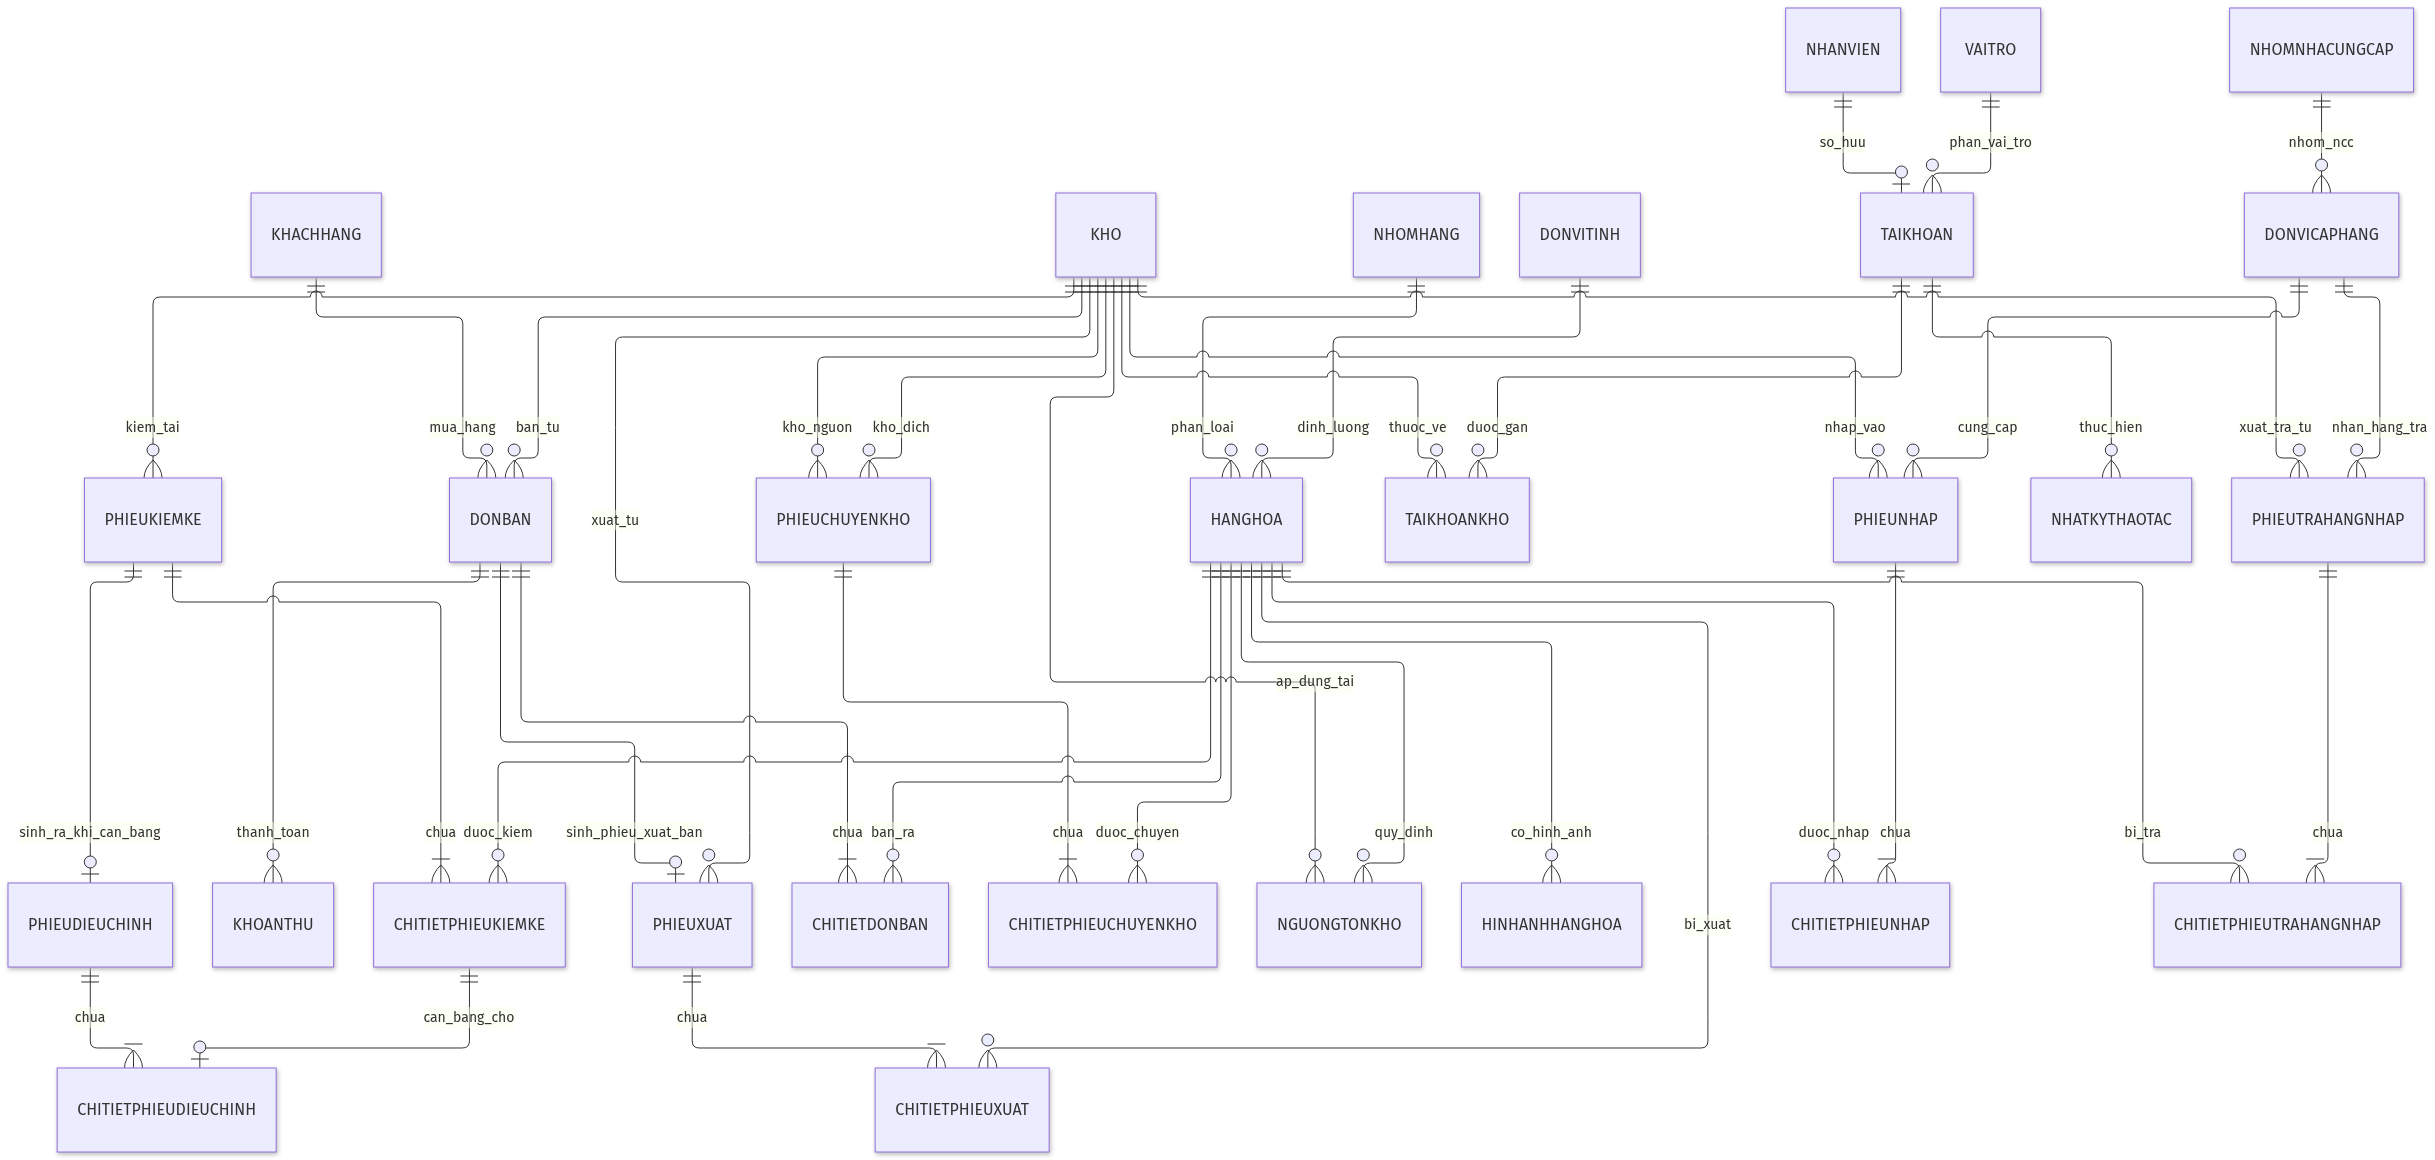
\includegraphics[width=0.98\textwidth, height=11.5cm, keepaspectratio]{figures/fig_er_tong_quan.png}
\caption{Mô hình thực thể -- liên kết tổng quát (Sơ đồ ER - Entity-Relationship Diagram)}
\label{fig:so_do_er}
\end{figure}

\subsubsection{Các sơ đồ ER phân rã chi tiết theo cụm nghiệp vụ}

Để thể hiện trực quan đầy đủ cấu trúc thuộc tính, kiểu dữ liệu, các ràng buộc khóa (PK, FK, UK) và bản số tham gia (Crow's Foot Notation) chính xác như trong tài liệu đặc tả, hệ thống được phân rã thành 5 sơ đồ cụm nghiệp vụ:

\clearpage
\begin{figure}[H]
\centering
{\bfseries\large a) Cụm 1: Quản trị Hệ thống, Nhân sự \& Phân quyền kho (RBAC)}\par\vspace{0.3cm}
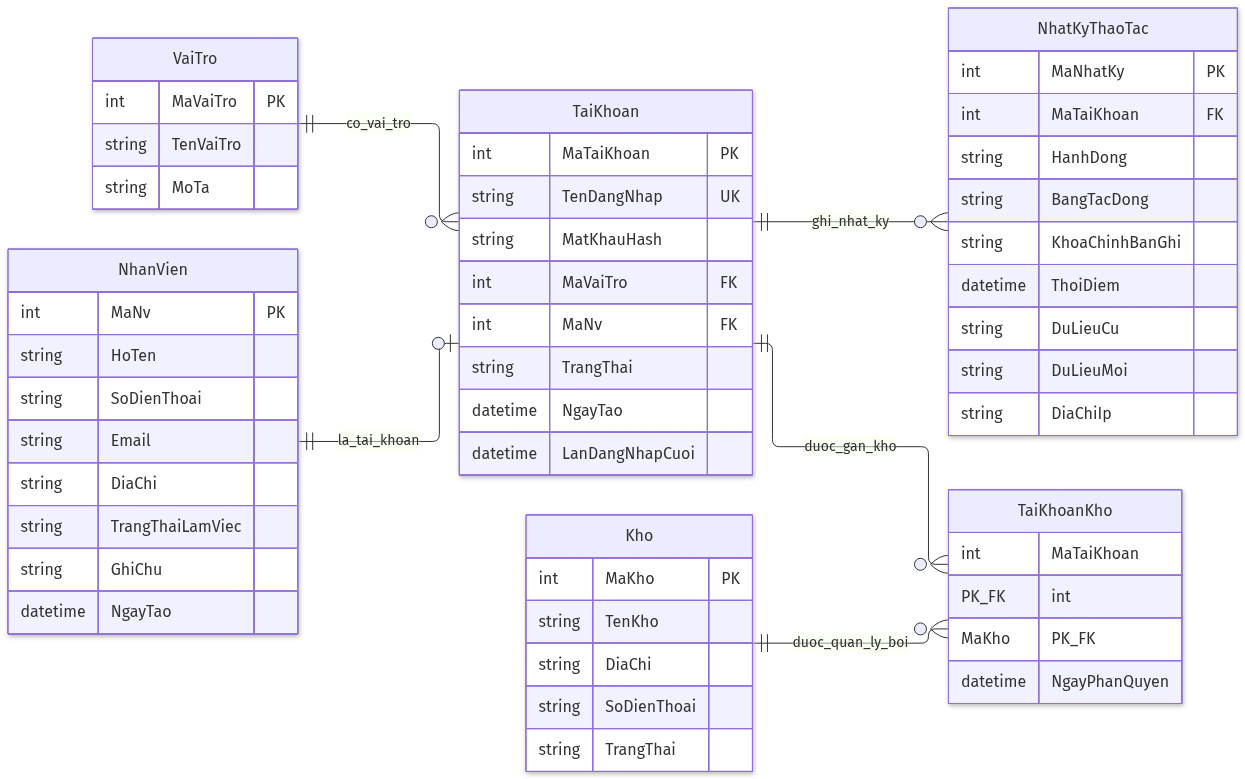
\includegraphics[width=0.92\textwidth, height=13cm, keepaspectratio]{figures/fig_er_rbac.png}
\vspace{0.2cm}
\caption{Sơ đồ ER Cụm Quản trị Hệ thống, Nhân sự \& Phân quyền kho (RBAC)}
\label{fig:er_rbac}
\end{figure}

\clearpage
\begin{figure}[H]
\centering
{\bfseries\large b) Cụm 2: Danh mục Hàng hóa, Định mức tồn \& Đơn vị tính}\par\vspace{0.3cm}
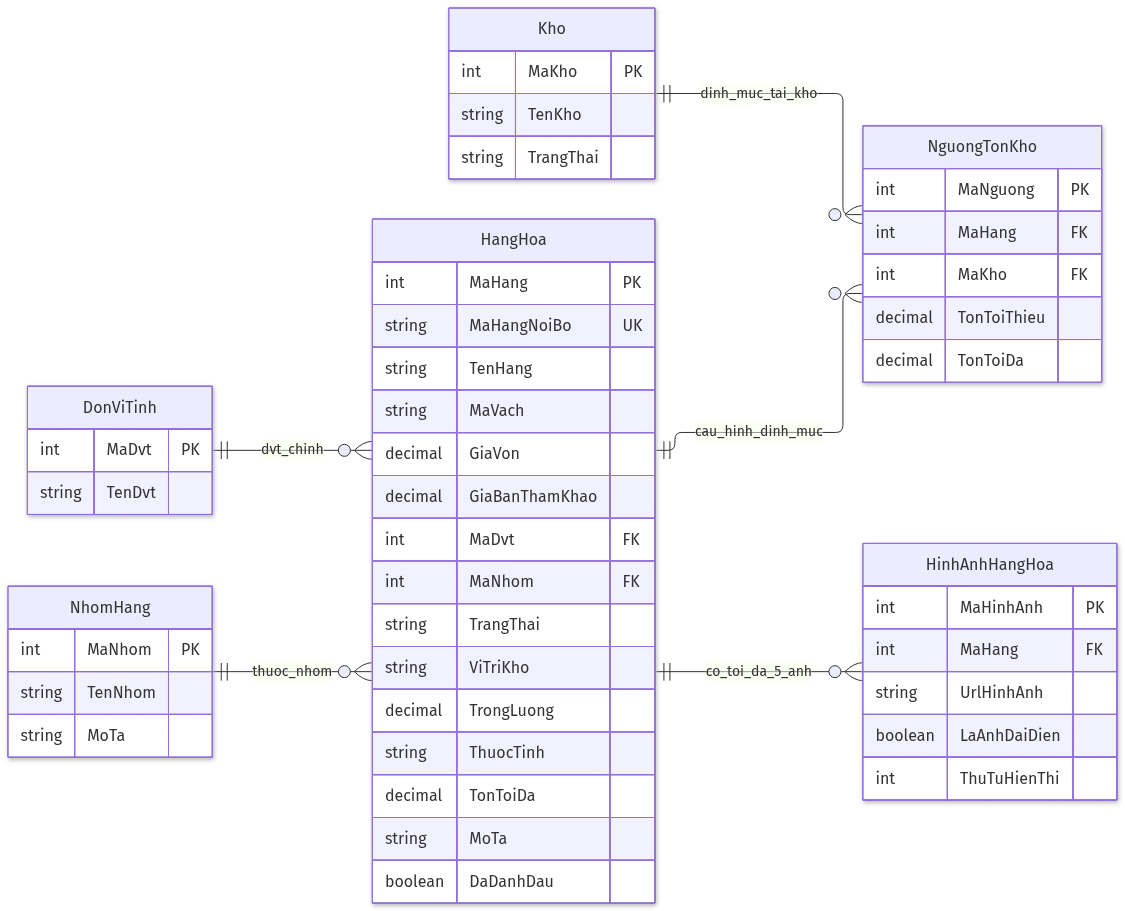
\includegraphics[width=0.92\textwidth, height=13cm, keepaspectratio]{figures/fig_er_hanghoa.png}
\vspace{0.2cm}
\caption{Sơ đồ ER Cụm Danh mục Hàng hóa, Định mức tồn \& Đơn vị tính}
\label{fig:er_hanghoa}
\end{figure}

\clearpage
\begin{figure}[H]
\centering
{\bfseries\large c) Cụm 3: Chuỗi cung ứng (Nhập hàng \& Trả hàng Nhà cung cấp)}\par\vspace{0.3cm}
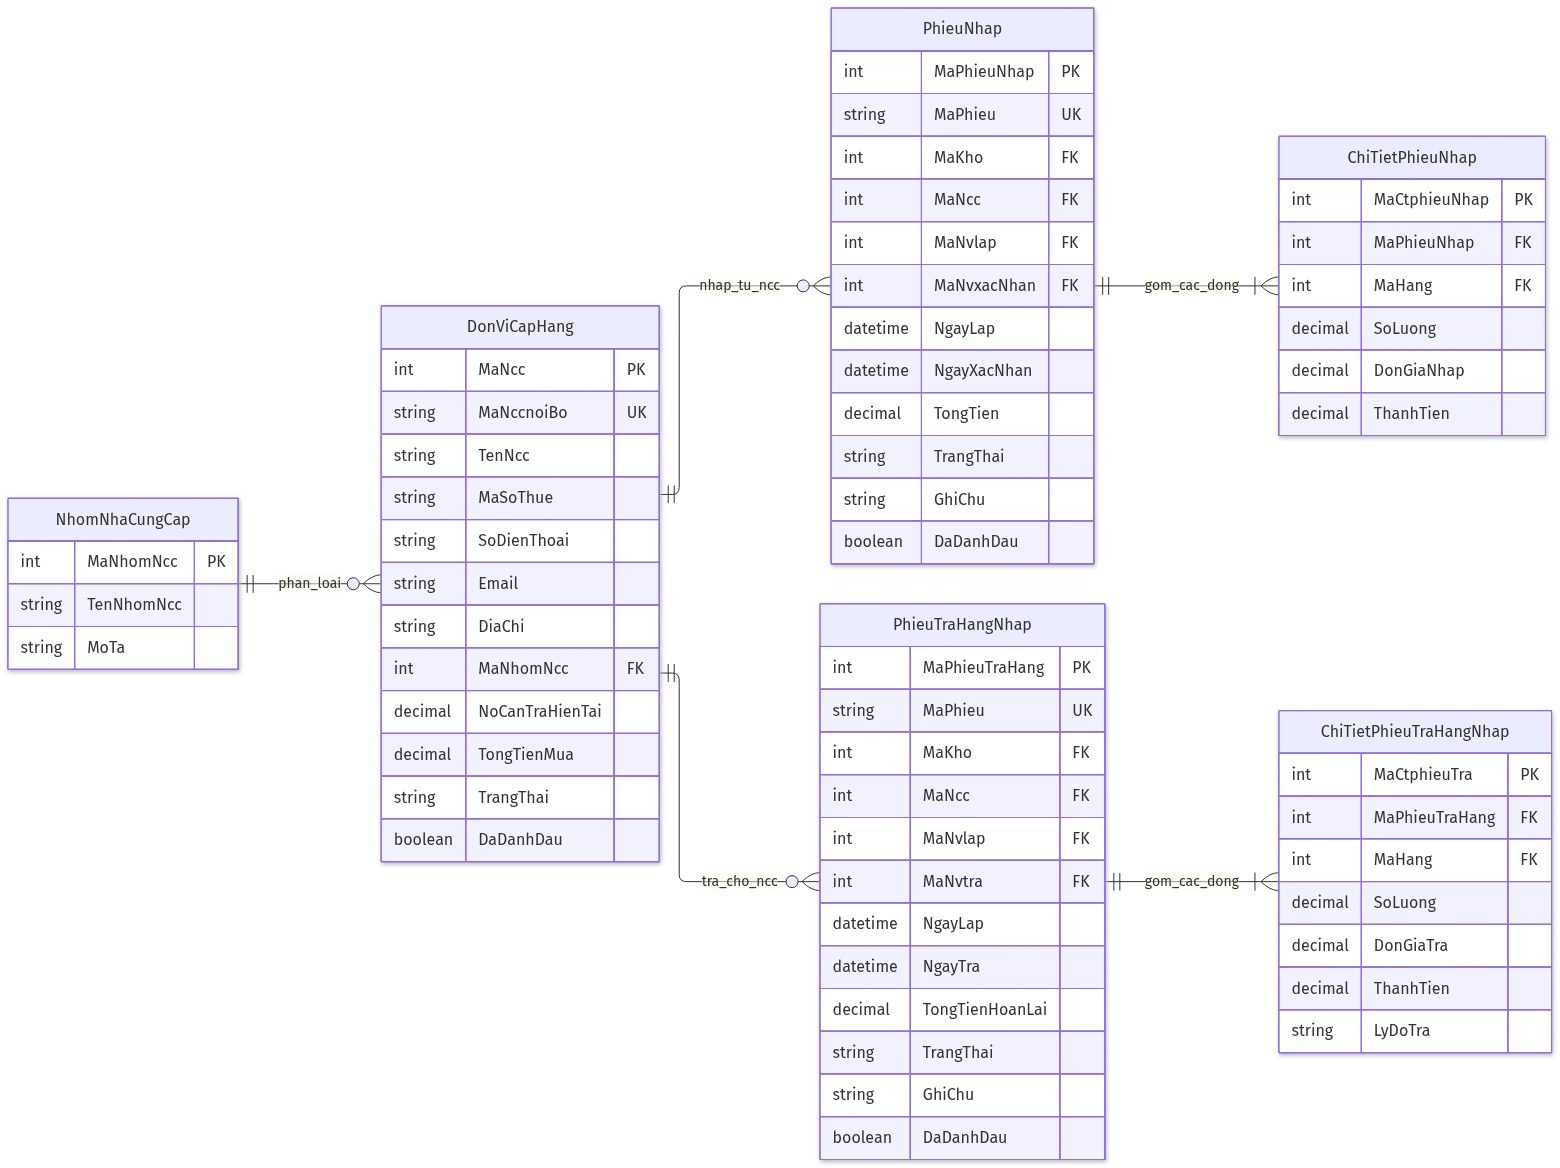
\includegraphics[width=0.95\textwidth, height=13cm, keepaspectratio]{figures/fig_er_supply_chain.png}
\vspace{0.2cm}
\caption{Sơ đồ ER Cụm Chuỗi cung ứng Nhập kho \& Xuất trả nhà cung cấp}
\label{fig:er_supply_chain}
\end{figure}

\clearpage
\begin{figure}[H]
\centering
{\bfseries\large d) Cụm 4: Luân chuyển nội bộ, Xuất hủy \& Kiểm kê - Cân bằng kho}\par\vspace{0.3cm}
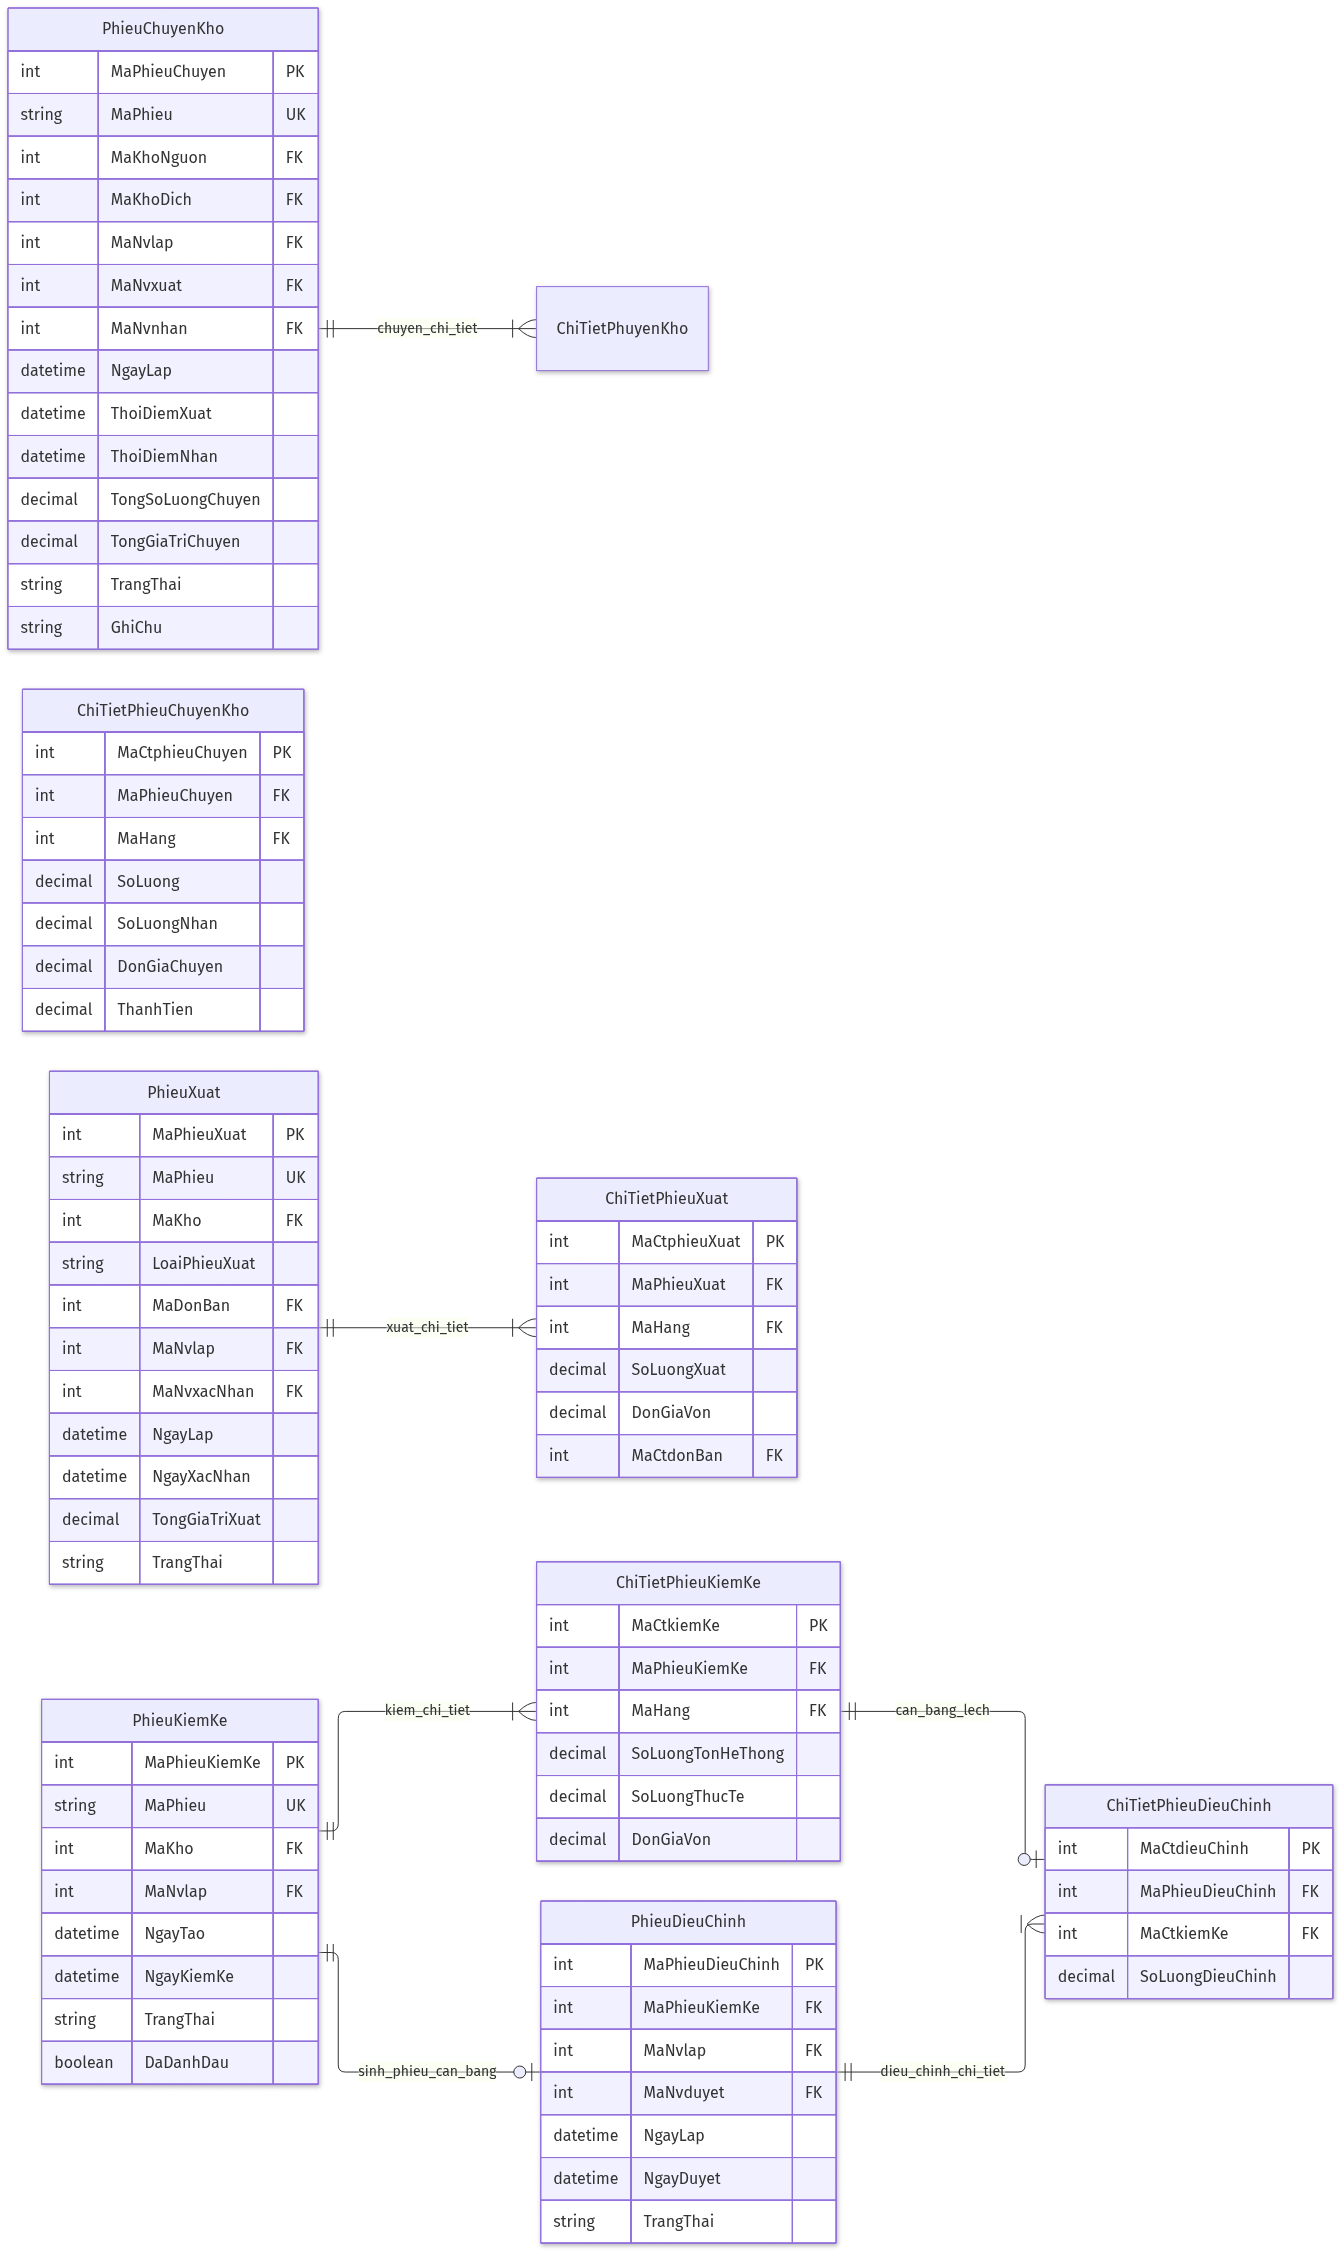
\includegraphics[width=0.90\textwidth, height=13.5cm, keepaspectratio]{figures/fig_er_transfer_audit.png}
\vspace{0.2cm}
\caption{Sơ đồ ER Cụm Điều chuyển kho, Xuất hủy \& Kiểm kê cân bằng kho}
\label{fig:er_transfer_audit}
\end{figure}

\clearpage
\begin{figure}[H]
\centering
{\bfseries\large e) Cụm 5: Bán hàng \& Quản lý dòng tiền (Khách hàng \& Khoản thu)}\par\vspace{0.3cm}
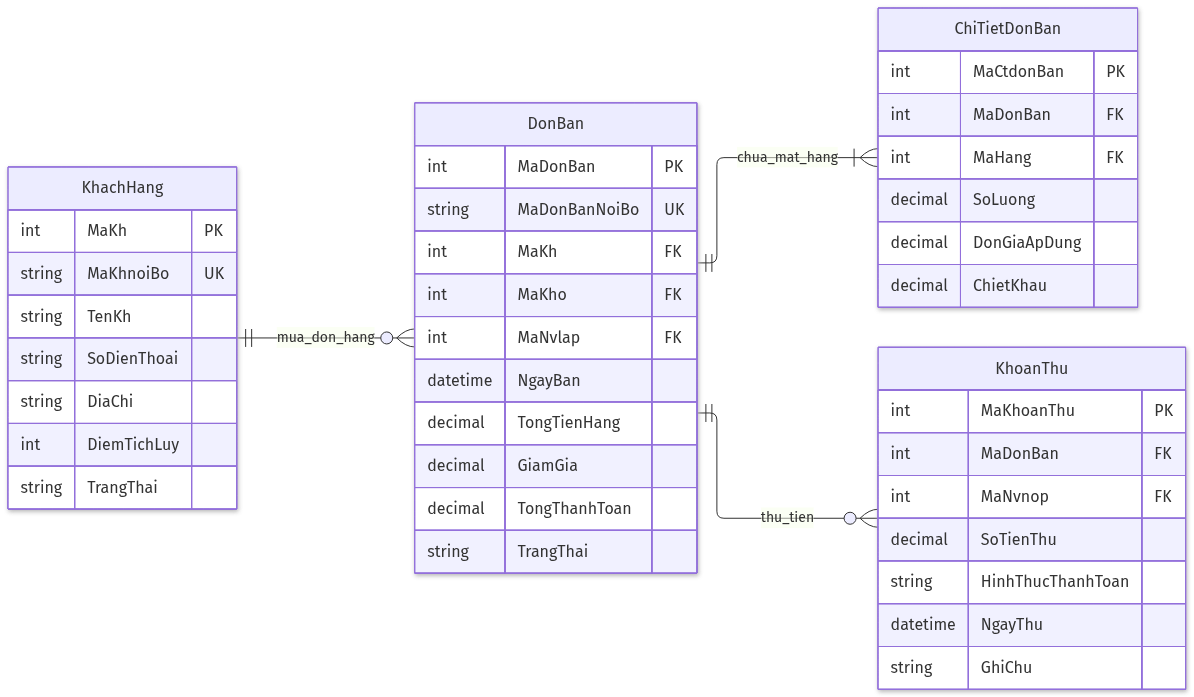
\includegraphics[width=0.92\textwidth, height=12.5cm, keepaspectratio]{figures/fig_er_sales.png}
\vspace{0.2cm}
\caption{Sơ đồ ER Cụm Đơn bán hàng \& Quản lý khoản thu}
\label{fig:er_sales}
\end{figure}
\clearpage

\subsection{Mô hình dữ liệu quan hệ (Sơ đồ RM - Relational Model)}
Áp dụng các quy tắc chuyển đổi từ mô hình ER sang mô hình quan hệ (Mapping ER to Relational Model), hệ thống chuẩn hóa cơ sở dữ liệu đạt chuẩn dạng chuẩn 3 (3NF) nhằm loại bỏ dư thừa dữ liệu và ngăn ngừa dị thường thao tác.

\subsubsection{Lược đồ quan hệ chuẩn (Relational Schema Notation)}
Quy ước ký hiệu: Tên bảng ( \underline{Khóa chính PK}, Thuộc tính thường, \textit{Khóa ngoại FK*}, ... ) phân định theo 5 nhóm nghiệp vụ:

\textbf{a) Nhóm 1: Quản trị hệ thống \& Phân quyền kho (RBAC)}
\begin{enumerate}[label={\textbf{\arabic*./}}]
    \item \textbf{VaiTro} (\underline{MaVaiTro}, TenVaiTro, MoTa)
    \item \textbf{NhanVien} (\underline{MaNv}, HoTen, SoDienThoai, Email, DiaChi, TrangThaiLamViec, GhiChu, NgayTao)
    \item \textbf{TaiKhoan} (\underline{MaTaiKhoan}, TenDangNhap, MatKhauHash, \textit{MaVaiTro*}, \textit{MaNv*}, TrangThai, NgayTao, LanDangNhapCuoi)
    \item \textbf{TaiKhoan\_Kho} (\underline{MaTaiKhoan*, MaKho*}, NgayPhanQuyen)
    \item \textbf{NhatKyThaoTac} (\underline{MaNhatKy}, \textit{MaTaiKhoan*}, HanhDong, BangTacDong, KhoaChinhBanGhi, ThoiDiem, DuLieuCu, DuLieuMoi, DiaChiIp)
\end{enumerate}

\textbf{b) Nhóm 2: Danh mục hàng hóa, định mức \& kho hàng}
\begin{enumerate}[resume, label={\textbf{\arabic*./}}]
    \item \textbf{Kho} (\underline{MaKho}, TenKho, DiaChi, SoDienThoai, TrangThai, NgayTao)
    \item \textbf{DonViTinh} (\underline{MaDvt}, TenDvt)
    \item \textbf{NhomHang} (\underline{MaNhom}, TenNhom, MoTa)
    \item \textbf{HangHoa} (\underline{MaHang}, MaHangNoiBo, TenHang, MaVach, GiaVon, GiaBanThamKhao, \textit{MaDvt*}, \textit{MaNhom*}, TrangThai, ViTriKho, TrongLuong, ThuocTinh, TonToiDa, MoTa, DaDanhDau, NgayTao, NgayCapNhat)
    \item \textbf{HinhAnhHangHoa} (\underline{MaHinhAnh}, \textit{MaHang*}, UrlHinhAnh, LaAnhDaiDien, ThuTuHienThi)
    \item \textbf{NguongTonKho} (\underline{MaNguong}, \textit{MaHang*}, \textit{MaKho*}, TonToiThieu, TonToiDa)
\end{enumerate}

\textbf{c) Nhóm 3: Đối tác \& Khách hàng}
\begin{enumerate}[resume, label={\textbf{\arabic*./}}]
    \item \textbf{NhomNhaCungCap} (\underline{MaNhomNcc}, TenNhomNcc, MoTa)
    \item \textbf{DonViCapHang} (\underline{MaNcc}, MaNccNoiBo, TenNcc, MaSoThue, SoDienThoai, Email, DiaChi, \textit{MaNhomNcc*}, NoCanTraHienTai, TongTienMua, TrangThai, DaDanhDau, NgayTao)
    \item \textbf{KhachHang} (\underline{MaKh}, MaKhNoiBo, TenKh, SoDienThoai, DiaChi, DiemTichLuy, TrangThai)
\end{enumerate}

\textbf{d) Nhóm 4: Giao dịch chứng từ nhập, xuất, chuyển, kiểm, trả hàng}
\begin{enumerate}[resume, label={\textbf{\arabic*./}}]
    \item \textbf{PhieuNhap} (\underline{MaPhieuNhap}, MaPhieu, \textit{MaKho*}, \textit{MaNcc*}, \textit{MaNvLap*}, \textit{MaNvXacNhan*}, NgayLap, NgayXacNhan, TongTien, TrangThai, GhiChu, DaDanhDau)
    \item \textbf{ChiTietPhieuNhap} (\underline{MaCtphieuNhap}, \textit{MaPhieuNhap*}, \textit{MaHang*}, SoLuong, DonGiaNhap, ThanhTien)
    \item \textbf{PhieuTraHangNhap} (\underline{MaPhieuTraHang}, MaPhieu, \textit{MaKho*}, \textit{MaNcc*}, \textit{MaNvLap*}, \textit{MaNvTra*}, NgayLap, NgayTra, TongTienHoanLai, TrangThai, GhiChu, DaDanhDau)
    \item \textbf{ChiTietPhieuTraHangNhap} (\underline{MaCtphieuTra}, \textit{MaPhieuTraHang*}, \textit{MaHang*}, SoLuong, DonGiaTra, ThanhTien, LyDoTra)
    \item \textbf{PhieuXuat} (\underline{MaPhieuXuat}, MaPhieu, \textit{MaKho*}, LoaiPhieuXuat, \textit{MaDonBan*}, \textit{MaNvLap*}, \textit{MaNvXacNhan*}, NgayLap, NgayXacNhan, TongGiaTriXuat, TrangThai, GhiChu, DaDanhDau)
    \item \textbf{ChiTietPhieuXuat} (\underline{MaCtphieuXuat}, \textit{MaPhieuXuat*}, \textit{MaHang*}, SoLuongXuat, DonGiaVon, \textit{MaCtdonBan*})
    \item \textbf{PhieuChuyenKho} (\underline{MaPhieuChuyen}, MaPhieu, \textit{MaKhoNguon*}, \textit{MaKhoDich*}, \textit{MaNvLap*}, \textit{MaNvXuat*}, \textit{MaNvNhan*}, NgayLap, ThoiDiemXuat, ThoiDiemNhan, TongSoLuongChuyen, TongGiaTriChuyen, TrangThai, GhiChu, DaDanhDau)
    \item \textbf{ChiTietPhieuChuyenKho} (\underline{MaCtphieuChuyen}, \textit{MaPhieuChuyen*}, \textit{MaHang*}, SoLuong, SoLuongNhan, DonGiaChuyen, ThanhTien)
    \item \textbf{PhieuKiemKe} (\underline{MaPhieuKiemKe}, MaPhieu, \textit{MaKho*}, \textit{MaNvLap*}, NgayTao, NgayKiemKe, TrangThai, GhiChu, DaDanhDau)
    \item \textbf{ChiTietPhieuKiemKe} (\underline{MaCtkiemKe}, \textit{MaPhieuKiemKe*}, \textit{MaHang*}, SoLuongTonHeThong, SoLuongThucTe, DonGiaVon, GhiChu)
    \item \textbf{PhieuDieuChinh} (\underline{MaPhieuDieuChinh}, \textit{MaPhieuKiemKe*}, \textit{MaNvLap*}, \textit{MaNvDuyet*}, NgayLap, NgayDuyet, LyDoDieuChinh, TrangThai)
    \item \textbf{ChiTietPhieuDieuChinh} (\underline{MaCtdieuChinh}, \textit{MaPhieuDieuChinh*}, \textit{MaCtkiemKe*}, SoLuongDieuChinh, GhiChu)
\end{enumerate}

\textbf{e) Nhóm 5: Đơn bán lẻ \& Quản lý dòng tiền}
\begin{enumerate}[resume, label={\textbf{\arabic*./}}]
    \item \textbf{DonBan} (\underline{MaDonBan}, MaDonBanNoiBo, \textit{MaKh*}, \textit{MaKho*}, \textit{MaNvLap*}, NgayBan, TongTienHang, GiamGia, TongThanhToan, TrangThai, GhiChu)
    \item \textbf{ChiTietDonBan} (\underline{MaCtdonBan}, \textit{MaDonBan*}, \textit{MaHang*}, SoLuong, DonGiaApDung, ChietKhau)
    \item \textbf{KhoanThu} (\underline{MaKhoanThu}, \textit{MaDonBan*}, \textit{MaNvNop*}, SoTienThu, HinhThucThanhToan, NgayThu, GhiChu)
\end{enumerate}

\subsubsection{Sơ đồ cấu trúc liên kết các bảng quan hệ (Sơ đồ RM vật lý)}
Hình~\ref{fig:so_do_rm} thể hiện Sơ đồ quan hệ RM với các bảng vật lý, khóa chính (PK) được gạch chân và các mũi tên chỉ rõ ràng buộc khóa ngoại (Foreign Key) tham chiếu về khóa chính của bảng cha:

\begin{figure}[H]
\centering
\begin{tikzpicture}[
    table/.style={draw=black, line width=0.8pt, rounded corners=2pt, fill=gray!5, inner sep=4pt, align=left, font=\scriptsize},
    pk/.style={font=\scriptsize\bfseries\underline},
    fk/.style={font=\scriptsize\itshape},
    ref/.style={->, thick, black}
]
    % Hàng 1: Danh mục nền tảng
    \node[table] (dvt) at (0, 4) {
        \textbf{DonViTinh}\\
        \underline{MaDvt} (PK)\\
        TenDvt
    };

    \node[table] (nhom) at (4, 4) {
        \textbf{NhomHang}\\
        \underline{MaNhom} (PK)\\
        TenNhom
    };

    \node[table] (kho) at (9.5, 4) {
        \textbf{Kho}\\
        \underline{MaKho} (PK)\\
        TenKho\\
        DiaChi, TrangThai
    };

    % Hàng 2: Hàng hóa & Người dùng
    \node[table] (hh) at (2, 1.2) {
        \textbf{HangHoa}\\
        \underline{MaHang} (PK)\\
        MaHangNoiBo (UQ)\\
        TenHang, MaVach\\
        GiaVon, GiaBan\\
        \textit{MaDvt} (FK), \textit{MaNhom} (FK)
    };

    \node[table] (ncc) at (-2.5, 1.2) {
        \textbf{DonViCapHang}\\
        \underline{MaNcc} (PK)\\
        TenNcc, DienThoai
    };

    \node[table] (tk) at (9.5, 1.2) {
        \textbf{TaiKhoan}\\
        \underline{MaTaiKhoan} (PK)\\
        TenDangNhap, HoTen\\
        \textit{MaVaiTro} (FK)
    };

    % Hàng 3: Chứng từ Master
    \node[table] (pn) at (-1.5, -2) {
        \textbf{PhieuNhap}\\
        \underline{MaPhieuNhap} (PK)\\
        MaPhieu (UQ), NgayNhap\\
        \textit{MaKho} (FK), \textit{MaNcc} (FK)\\
        TongTien, TrangThai
    };

    \node[table] (pkk) at (6, -2) {
        \textbf{PhieuKiemKe}\\
        \underline{MaPhieuKiem} (PK)\\
        MaPhieu (UQ), NgayKiemKe\\
        \textit{MaKho} (FK), TrangThai
    };

    % Hàng 4: Chi tiết Detail
    \node[table] (ctpn) at (-1.5, -4.8) {
        \textbf{ChiTietPhieuNhap}\\
        \underline{MaChiTiet} (PK)\\
        \textit{MaPhieuNhap} (FK)\\
        \textit{MaHang} (FK)\\
        SoLuong, DonGia
    };

    \node[table] (ctkk) at (6, -4.8) {
        \textbf{ChiTietPhieuKiemKe}\\
        \underline{MaChiTiet} (PK)\\
        \textit{MaPhieuKiem} (FK)\\
        \textit{MaHang} (FK)\\
        SoLuongThucTe, SoLuongTon
    };

    % Các đường liên kết FK -> PK
    \draw[ref] (hh.north) -- ++(0, 0.5) -| (dvt.south);
    \draw[ref] (hh.north) -- ++(0, 0.5) -| (nhom.south);

    \draw[ref] (pn.north) -- ++(0, 0.5) -| (ncc.south);
    \draw[ref] (pn.east) -- ++(1, 0) |- (kho.west);

    \draw[ref] (pkk.north) -- (kho.south);

    \draw[ref] (ctpn.north) -- (pn.south);
    \draw[ref] (ctpn.east) -| (hh.south);

    \draw[ref] (ctkk.north) -- (pkk.south);
    \draw[ref] (ctkk.west) -| (hh.south);
\end{tikzpicture}
\caption{Sơ đồ cấu trúc liên kết các bảng quan hệ (Sơ đồ RM - Relational Model)}
\label{fig:so_do_rm}
\end{figure}

\subsubsection{Bảng các ràng buộc toàn vẹn tham chiếu (Referential Integrity Constraints)}
Các ràng buộc khóa ngoại (Foreign Key) đảm bảo tính toàn vẹn tham chiếu giữa các quan hệ theo công thức toán học: $\pi_{FK}(R) \subseteq \pi_{PK}(S)$. Bảng~\ref{tab:fk_constraints} thống kê các ràng buộc tham chiếu cốt lõi trong hệ thống:

\begin{table}[H]
\centering
\footnotesize
\renewcommand{\arraystretch}{1.05}
\begin{tabularx}{\textwidth}{|p{3.5cm}|p{2.6cm}|p{2.0cm}|p{2.6cm}|p{2.0cm}|Y|}
\hline
\rowcolor{tableheader}
\textbf{Tên ràng buộc} & \textbf{Bảng tham chiếu ($R$)} & \textbf{Khóa ngoại ($FK$)} & \textbf{Bảng cha ($S$)} & \textbf{Khóa chính ($PK$)} & \textbf{Hành vi xóa} \\
\hline
FK\_TaiKhoan\_VaiTro & TaiKhoan & MaVaiTro & VaiTro & MaVaiTro & NO ACTION \\
\hline
FK\_TaiKhoan\_NhanVien & TaiKhoan & MaNv & NhanVien & MaNv & SET NULL \\
\hline
FK\_TaiKhoanKho\_TaiKhoan & TaiKhoanKho & MaTaiKhoan & TaiKhoan & MaTaiKhoan & CASCADE \\
\hline
FK\_TaiKhoanKho\_Kho & TaiKhoanKho & MaKho & Kho & MaKho & CASCADE \\
\hline
FK\_HangHoa\_DonViTinh & HangHoa & MaDvt & DonViTinh & MaDvt & NO ACTION \\
\hline
FK\_HangHoa\_NhomHang & HangHoa & MaNhom & NhomHang & MaNhom & NO ACTION \\
\hline
FK\_HinhAnh\_HangHoa & HinhAnhHangHoa & MaHang & HangHoa & MaHang & CASCADE \\
\hline
FK\_NguongTon\_Kho & NguongTonKho & MaKho & Kho & MaKho & CASCADE \\
\hline
FK\_PhieuNhap\_Kho & PhieuNhap & MaKho & Kho & MaKho & NO ACTION \\
\hline
FK\_PhieuNhap\_NCC & PhieuNhap & MaNcc & DonViCapHang & MaNcc & NO ACTION \\
\hline
FK\_CTPN\_PhieuNhap & ChiTietPhieuNhap & MaPhieuNhap & PhieuNhap & MaPhieuNhap & CASCADE \\
\hline
FK\_CTPN\_HangHoa & ChiTietPhieuNhap & MaHang & HangHoa & MaHang & NO ACTION \\
\hline
FK\_PhieuTra\_Kho & PhieuTraHangNhap & MaKho & Kho & MaKho & NO ACTION \\
\hline
FK\_CTPT\_PhieuTra & ChiTietPhieuTra & MaPhieuTra & PhieuTraHangNhap & MaPhieuTra & CASCADE \\
\hline
FK\_ChuyenKho\_KhoNguon & PhieuChuyenKho & MaKhoNguon & Kho & MaKho & NO ACTION \\
\hline
FK\_CTPCK\_PhieuChuyen & ChiTietPhieuChuyen & MaPhieuChuyen & PhieuChuyenKho & MaPhieuChuyen & CASCADE \\
\hline
FK\_PhieuKiem\_Kho & PhieuKiemKe & MaKho & Kho & MaKho & NO ACTION \\
\hline
FK\_CTPKK\_PhieuKiem & ChiTietPhieuKiem & MaPhieuKiem & PhieuKiemKe & MaPhieuKiem & CASCADE \\
\hline
FK\_DieuChinh\_PhieuKiem & PhieuDieuChinh & MaPhieuKiem & PhieuKiemKe & MaPhieuKiem & NO ACTION \\
\hline
FK\_DonBan\_KhachHang & DonBan & MaKh & KhachHang & MaKh & NO ACTION \\
\hline
FK\_CTDB\_DonBan & ChiTietDonBan & MaDonBan & DonBan & MaDonBan & CASCADE \\
\hline
\end{tabularx}
\caption{Bảng các ràng buộc toàn vẹn tham chiếu trọng tâm trong cơ sở dữ liệu}
\label{tab:fk_constraints}
\end{table}

\subsubsection{Đánh giá chuẩn hóa cơ sở dữ liệu (3NF / BCNF)}
Cơ sở dữ liệu \texttt{QuanLyKhoPhuQuocLTW} được thiết kế tuân thủ nghiêm ngặt lý thuyết chuẩn hóa quan hệ nhằm triệt tiêu dư thừa dữ liệu và chống dị thường (Anomalies):
\begin{enumerate}
    \item \textbf{Dạng chuẩn 1 (1NF):} Toàn bộ các thuộc tính trong các quan hệ đều là thuộc tính nguyên tố (Atomic values), không chứa tập giá trị lặp. Các thuộc tính đa trị (như danh sách ảnh sản phẩm) được tách ra quan hệ riêng \texttt{HinhAnhHangHoa}; định mức tồn kho phân tán theo chi nhánh được tách thành \texttt{NguongTonKho}.
    \item \textbf{Dạng chuẩn 2 (2NF):} Đạt 1NF và mọi thuộc tính không khóa đều phụ thuộc hàm đầy đủ vào khóa chính. Đối với bảng có khóa chính hỗn hợp như \texttt{TaiKhoan\_Kho(MaTaiKhoan, MaKho)}, thuộc tính \texttt{NgayPhanQuyen} phụ thuộc hàm vào toàn bộ cặp khóa chính, không phụ thuộc vào một phần khóa.
    \item \textbf{Dạng chuẩn 3 (3NF) \& BCNF:} Đạt 2NF và không tồn tại bất kỳ phụ thuộc hàm bắc cầu nào giữa các thuộc tính không khóa ($X \rightarrow Y \rightarrow Z$). Ví dụ: Thông tin nhân viên không lưu trong bảng \texttt{TaiKhoan} mà được tách riêng thành bảng \texttt{NhanVien}; thông tin nhà cung cấp không lưu dư thừa trong \texttt{PhieuNhap} mà tham chiếu khóa ngoại tới \texttt{DonViCapHang}.
    \item \textbf{Phi vật lý hóa số lượng tồn kho (Dynamic Inventory Engine):} Điểm đặc sắc nhất trong thiết kế là việc \textbf{loại bỏ hoàn toàn thuộc tính tồn kho tĩnh} trên bảng vật lý \texttt{HangHoa}. Toàn bộ số lượng tồn kho được tính toán động theo thời gian thực qua Database View \texttt{vw\_TonKhoHienTai}, ngăn chặn triệt để tình trạng bất đồng bộ dữ liệu (Race Condition) và tranh chấp khóa khi nhiều người dùng thao tác đồng thời.
\end{enumerate}

\subsection{Từ điển dữ liệu chi tiết các bảng chính}

Dưới đây là từ điển dữ liệu kỹ thuật của các thực thể cốt lõi trong hệ thống:

\begin{table}[H]
\centering
\small
\renewcommand{\arraystretch}{1.15}
\begin{tabularx}{\textwidth}{|p{2.8cm}|p{3.2cm}|c|c|Y|}
\hline
\rowcolor{tableheader}
\textbf{Tên cột} & \textbf{Kiểu dữ liệu} & \textbf{Khóa} & \textbf{Null} & \textbf{Mô tả / Ràng buộc} \\
\hline
MaHang & INT IDENTITY(1,1) & PK & No & Mã định danh tự tăng duy nhất hàng hóa \\
\hline
MaHangNoiBo & NVARCHAR(50) & Unique & No & Mã SKU hàng hóa (VD: HH0001, SP002) \\
\hline
TenHang & NVARCHAR(250) & & No & Tên hiển thị đầy đủ của mặt hàng \\
\hline
MaVach & VARCHAR(50) & Index & Yes & Mã vạch barcode quét nhanh khi thao tác \\
\hline
GiaVon & DECIMAL(18,2) & & No & Giá vốn bình quân gia quyền tính tự động \\
\hline
GiaBanThamKhao & DECIMAL(18,2) & & No & Giá bán niêm yết tham khảo \\
\hline
ViTriKho & NVARCHAR(100) & & Yes & Vị trí lưu kho (Kệ / Dãy / Tầng) \\
\hline
TrongLuong & DECIMAL(18,2) & & Yes & Trọng lượng đơn vị hàng hóa (gam) \\
\hline
TonToiDa & DECIMAL(18,2) & & Yes & Định mức tồn tối đa cảnh báo đọng vốn \\
\hline
MaDvt & INT & FK & No & Tham chiếu DonViTinh(MaDvt) \\
\hline
MaNhom & INT & FK & Yes & Tham chiếu NhomHang(MaNhom) \\
\hline
TrangThai & NVARCHAR(50) & & No & DANG\_KINH\_DOANH / NGUNG\_KD \\
\hline
\end{tabularx}
\caption{Từ điển dữ liệu bảng HangHoa (Hàng hóa)}
\label{tab:dict_hanghoa}
\end{table}

\begin{table}[H]
\centering
\small
\renewcommand{\arraystretch}{1.15}
\begin{tabularx}{\textwidth}{|p{2.8cm}|p{3.2cm}|c|c|Y|}
\hline
\rowcolor{tableheader}
\textbf{Tên cột} & \textbf{Kiểu dữ liệu} & \textbf{Khóa} & \textbf{Null} & \textbf{Mô tả / Ràng buộc} \\
\hline
MaKho & INT IDENTITY(1,1) & PK & No & Mã định danh duy nhất chi nhánh kho \\
\hline
TenKho & NVARCHAR(200) & Unique & No & Tên chi nhánh kho (Kho Tổng, Kho 2...) \\
\hline
DiaChi & NVARCHAR(300) & & Yes & Địa chỉ thực tế của chi nhánh kho \\
\hline
SoDienThoai & VARCHAR(20) & & Yes & Số điện thoại hotline liên hệ chi nhánh \\
\hline
TrangThai & NVARCHAR(50) & & No & HOAT\_DONG / NGUNG\_HOAT\_DONG \\
\hline
\end{tabularx}
\caption{Từ điển dữ liệu bảng Kho (Chi nhánh kho vật lý)}
\label{tab:dict_kho}
\end{table}

\begin{table}[H]
\centering
\small
\renewcommand{\arraystretch}{1.15}
\begin{tabularx}{\textwidth}{|p{2.8cm}|p{3.2cm}|c|c|Y|}
\hline
\rowcolor{tableheader}
\textbf{Tên cột} & \textbf{Kiểu dữ liệu} & \textbf{Khóa} & \textbf{Null} & \textbf{Mô tả / Ràng buộc} \\
\hline
MaPhieuNhap & INT IDENTITY(1,1) & PK & No & Khóa chính phiếu nhập kho \\
\hline
MaPhieu & NVARCHAR(50) & Unique & No & Mã hiển thị người dùng (VD: PN000001) \\
\hline
MaKho & INT & FK & No & Tham chiếu Kho(MaKho) nơi nhập hàng vào \\
\hline
MaNcc & INT & FK & No & Tham chiếu DonViCapHang(MaNcc) \\
\hline
TongTien & DECIMAL(18,2) & & No & Tổng giá trị lô hàng nhập từ NCC \\
\hline
TrangThai & NVARCHAR(50) & & No & PHIEU\_TAM / DA\_XAC\_NHAN / DA\_HUY \\
\hline
SoLuong & DECIMAL(18,2) & & No & Cột trong ChiTiet: Số lượng thực nhập \\
\hline
DonGiaNhap & DECIMAL(18,2) & & No & Cột trong ChiTiet: Đơn giá nhập thực tế \\
\hline
ThanhTien & DECIMAL(18,2) & & No & Cột trong ChiTiet: Thành tiền = SL $\times$ Đơn giá \\
\hline
\end{tabularx}
\caption{Từ điển dữ liệu bảng PhieuNhap \& ChiTietPhieuNhap}
\label{tab:dict_nhaphang}
\end{table}

\begin{table}[H]
\centering
\small
\renewcommand{\arraystretch}{1.15}
\begin{tabularx}{\textwidth}{|p{2.8cm}|p{3.2cm}|c|c|Y|}
\hline
\rowcolor{tableheader}
\textbf{Tên cột} & \textbf{Kiểu dữ liệu} & \textbf{Khóa} & \textbf{Null} & \textbf{Mô tả / Ràng buộc} \\
\hline
MaPhieuChuyen & INT IDENTITY(1,1) & PK & No & Khóa chính phiếu điều chuyển kho \\
\hline
MaPhieu & NVARCHAR(50) & Unique & No & Mã hiển thị (VD: CK000001) \\
\hline
MaKhoNguon & INT & FK & No & Tham chiếu Kho(MaKho) xuất hàng đi \\
\hline
MaKhoDich & INT & FK & No & Tham chiếu Kho(MaKho) tiếp nhận hàng \\
\hline
TrangThai & NVARCHAR(50) & & No & PHIEU\_TAM / DA\_CHUYEN / DA\_NHAN / DA\_HUY \\
\hline
SoLuong & DECIMAL(18,2) & & No & Cột trong ChiTiet: Số lượng xuất chuyển \\
\hline
SoLuongNhan & DECIMAL(18,2) & & Yes & Cột trong ChiTiet: Số lượng kho đích thực nhận \\
\hline
DonGiaChuyen & DECIMAL(18,2) & & No & Cột trong ChiTiet: Giá vốn hàng chuyển \\
\hline
\end{tabularx}
\caption{Từ điển dữ liệu bảng PhieuChuyenKho \& ChiTietPhieuChuyenKho}
\label{tab:dict_chuyenkho}
\end{table}

\begin{table}[H]
\centering
\small
\renewcommand{\arraystretch}{1.15}
\begin{tabularx}{\textwidth}{|p{2.8cm}|p{3.2cm}|c|c|Y|}
\hline
\rowcolor{tableheader}
\textbf{Tên cột} & \textbf{Kiểu dữ liệu} & \textbf{Khóa} & \textbf{Null} & \textbf{Mô tả / Ràng buộc} \\
\hline
MaPhieuKiemKe & INT IDENTITY(1,1) & PK & No & Khóa chính phiếu kiểm kê \\
\hline
MaPhieu & NVARCHAR(50) & Unique & No & Mã chứng từ hiển thị (VD: PK000001) \\
\hline
MaKho & INT & FK & No & Tham chiếu Kho(MaKho) thực hiện kiểm \\
\hline
NgayKiemKe & DATETIME & & No & Thời điểm lập đợt kiểm kê hàng hóa \\
\hline
TrangThai & NVARCHAR(50) & & No & PHIEU\_TAM / DA\_CAN\_BANG / DA\_HUY \\
\hline
GhiChu & NVARCHAR(500) & & Yes & Ghi chú đợt kiểm kê thực tế \\
\hline
SoLuongTonHeThong & DECIMAL(18,2) & & No & Cột trong ChiTiet: Tồn sổ sách lúc kiểm \\
\hline
SoLuongThucTe & DECIMAL(18,2) & & No & Cột trong ChiTiet: Số lượng thực đếm \\
\hline
DonGiaVon & DECIMAL(18,2) & & No & Cột trong ChiTiet: Giá vốn tính chênh lệch \\
\hline
\end{tabularx}
\caption{Từ điển dữ liệu bảng PhieuKiemKe \& ChiTietPhieuKiemKe}
\label{tab:dict_kiemkho}
\end{table}

\subsection{Giải thuật Database View 2 tầng tính toán tồn kho động}
Để loại bỏ hoàn toàn nguy cơ sai lệch tồn kho (Race Condition, Lost Updates) và đảm bảo tính toàn vẹn chứng từ theo chuẩn ERP, hệ thống áp dụng nguyên tắc kiến trúc: \textbf{Tuyệt đối không lưu cột số lượng tồn kho tĩnh trên bảng vật lý}. Toàn bộ số lượng tồn kho sổ sách được tính toán theo thời gian thực thông qua hệ thống Database View 2 tầng:

\begin{figure}[H]
\centering
\begin{tikzpicture}[
    node distance=1.1cm,
    block/.style={rectangle, draw=black, line width=0.8pt, fill=gray!6, rounded corners=2pt, text width=6cm, align=center, inner sep=5pt, font=\footnotesize},
    view/.style={rectangle, draw=black, line width=1pt, fill=blue!8, rounded corners=3pt, text width=7.2cm, align=center, inner sep=6pt, font=\small\bfseries},
    arrow/.style={->, thick, black}
]
    \node[block] (s1) {1. Phiếu Nhập hàng (DA\_XAC\_NHAN): + SL Nhập};
    \node[block, below=0.25cm of s1] (s2) {2. Phiếu Xuất hủy (DA\_XAC\_NHAN): - SL Xuất};
    \node[block, below=0.25cm of s2] (s3) {3. Chuyển kho (DA\_XUAT / DA\_NHAN): - SL Kho Nguồn};
    \node[block, below=0.25cm of s3] (s4) {4. Chuyển kho (DA\_NHAN): + SL Thực nhận Kho Đích};
    \node[block, below=0.25cm of s4] (s5) {5. Cân bằng kiểm kê (DA\_DUYET): $\pm$ SL Điều chỉnh};
    \node[block, below=0.25cm of s5] (s6) {6. Trả hàng nhập (DA\_TRA\_HANG): - SL Trả NCC};

    \node[view, right=1.6cm of s3] (v1) {TẦNG 1: View vw\_BienDongKho\\(Hợp nhất 6 dòng chứng từ thời gian thực:\\NgayGiaoDich, MaKho, MaHang, SL\_Tang, SL\_Giam)};

    \node[view, below=1.2cm of v1] (v2) {TẦNG 2: View vw\_TonKhoHienTai\\$\text{TonHienTai} = \sum \text{SL\_Tang} - \sum \text{SL\_Giam}$\\GROUP BY MaKho, MaHang};

    \draw[arrow] (s1.east) -- (v1.west);
    \draw[arrow] (s2.east) -- (v1.west);
    \draw[arrow] (s3.east) -- (v1.west);
    \draw[arrow] (s4.east) -- (v1.west);
    \draw[arrow] (s5.east) -- (v1.west);
    \draw[arrow] (s6.east) -- (v1.west);
    \draw[arrow] (v1) -- node[right, font=\footnotesize]{GROUP BY (Kho, Hàng)} (v2);
\end{tikzpicture}
\caption{Kiến trúc Database View 2 tầng tính toán tồn kho động}
\label{fig:view_2_tang}
\end{figure}

Công thức toán học của Tồn kho tức thời tại một chi nhánh kho:
\begin{equation}
\text{Tồn hiện tại}(h, k) = \sum \text{SốLượngTăng}(h, k) - \sum \text{SốLượngGiảm}(h, k)
\end{equation}

Nhờ kiến trúc 2 tầng này:
\begin{itemize}
    \item \textbf{Báo cáo Tồn kho (Pivot đa chi nhánh):} Truy vấn trực tiếp từ \texttt{vw\_TonKhoHienTai}, cho tốc độ phản hồi tính bằng mili-giây mà không cần tính toán thủ công ở tầng ứng dụng.
    \item \textbf{Báo cáo Thẻ kho:} Truy vấn từ \texttt{vw\_BienDongKho} theo khoảng thời gian $[TuNgay, DenNgay]$, cho phép tính tồn đầu kỳ chính xác tuyệt đối và tịnh tiến lũy kế từng giao dịch theo trình tự thời gian.
\end{itemize}

\section{Thiết kế Kiến trúc phần mềm và Giao diện người dùng}

\subsection{Mô hình kiến trúc MVC phân tầng trên ASP.NET Core}
Hệ thống được tổ chức theo mô hình kiến trúc MVC 3 tầng phân định trách nhiệm rõ ràng:
\begin{itemize}
    \item \textbf{Tầng Trình diễn (View / Presentation Layer):} Sử dụng Razor Views (\texttt{.cshtml}) kết hợp với Bootstrap 5, JavaScript ES6 và các khối Lego UI tái sử dụng.
    \item \textbf{Tầng Điều khiển \& Nghiệp vụ (Controller / Business Logic Layer):} Tiếp nhận các yêu cầu HTTP, kiểm tra ngữ cảnh chi nhánh qua \texttt{BaseKhoController}, thực thi xác thực quyền hạn và bọc giao dịch ACID.
    \item \textbf{Tầng Dữ liệu (Model / Data Access Layer):} Sử dụng Entity Framework Core 10 ánh xạ trực tiếp từ CSDL SQL Server thông qua \texttt{QuanLyKhoPhuQuocLtwContext}.
\end{itemize}

\subsection{Sơ đồ cấu trúc điều hướng trang (Sitemap)}
Luồng điều hướng người dùng được thiết kế khoa học:
Đăng nhập $\rightarrow$ Chọn chi nhánh kho $\rightarrow$ Dashboard tổng quan $\rightarrow$ Phân hệ Hàng hóa $\rightarrow$ Phân hệ Giao dịch (Nhập/Trả/Xuất/Chuyển/Kiểm) $\rightarrow$ Phân hệ Báo cáo (Tồn kho Pivot/Thẻ kho) $\rightarrow$ Thiết lập hệ thống (Kho/Người dùng).

\subsection{Thiết kế khung giao diện Wireframe chuẩn KiotViet}
Giao diện ứng dụng tuân thủ chuẩn mực giao diện 2 cột KiotViet:
\begin{itemize}
    \item \textbf{Thanh điều hướng cố định (Top Navbar):} Cao 42px, nền xanh KiotViet, chứa Logo, Menu điều hướng đa cấp, Dropdown chọn nhanh chi nhánh kho làm việc hiện hành và Thông tin tài khoản đăng nhập.
    \item \textbf{Sidebar Bộ lọc (Cột trái):} Chiều rộng 260px, gồm ô tìm kiếm nhanh F3, bộ lọc dải ngày \texttt{\_KiotDateFilter}, bộ lọc đa chọn kho \texttt{\_KiotMultiSelectFilter}, cây danh mục nhóm hàng và nút F4 thu gọn để mở rộng tối đa không gian làm việc.
    \item \textbf{Vùng làm việc chính (Cột phải):} Thanh công cụ chứa các nút tác vụ (+ Thêm mới, Xuất Excel, F1 Trợ giúp) và bảng dữ liệu hiển thị dạng bảng có hỗ trợ cuộn ngang và phân trang AJAX \texttt{\_Pagination}.
\end{itemize}

\cleardoublepage

% ==========================================
% CHƯƠNG 3: HIỆN THỰC HÓA VÀ LẬP TRÌNH HỆ THỐNG
% ==========================================
\chapter{HIỆN THỰC HÓA VÀ LẬP TRÌNH HỆ THỐNG}

\section{Môi trường công nghệ và công cụ phát triển}
Dự án được xây dựng và triển khai trên nền tảng công nghệ web hiện đại nhất hiện nay:
\begin{itemize}
    \item \textbf{Framework nền tảng:} ASP.NET Core MVC trên .NET 10 (\texttt{net10.0}) với ngôn ngữ C\# 13.
    \item \textbf{Truy xuất dữ liệu:} Entity Framework Core 10 theo chiến lược Database First, đảm bảo kiểm soát tuyệt đối cấu trúc SQL Server.
    \item \textbf{Hệ quản trị CSDL:} Microsoft SQL Server 2022 (CSDL \texttt{QuanLyKhoPhuQuocLTW}).
    \item \textbf{Công nghệ Front-end:} HTML5, CSS3, JavaScript ES6 thuần, Bootstrap 5.3, FontAwesome 6.
    \item \textbf{Thư viện xuất báo cáo:} ClosedXML hỗ trợ xuất tệp tin bảng tính Excel định dạng chuẩn XLSX.
\end{itemize}

\section{Xây dựng các cơ chế kiến trúc nền tảng (Core Framework)}

\subsection{Cơ chế Xác thực và Phân quyền theo Chi nhánh qua Cookie Authentication}
Hệ thống sử dụng cơ chế Cookie Authentication tích hợp sẵn của ASP.NET Core. Khi người dùng đăng nhập thành công, hệ thống cấp phát một Identity Cookie chứa các Claims danh tính:
\begin{lstlisting}[language={[Sharp]C}, caption={Thiết lập Claims danh tính và Chi nhánh làm việc trong AccountController}]
var claims = new List<Claim>
{
    new Claim(ClaimTypes.NameIdentifier, user.MaTaiKhoan.ToString()),
    new Claim(ClaimTypes.Name, user.TenDangNhap),
    new Claim(ClaimTypes.Role, user.MaVaiTroNavigation.TenVaiTro),
    new Claim("MaKhoMacDinh", selectedKhoId.ToString())
};
var claimsIdentity = new ClaimsIdentity(claims, CookieAuthenticationDefaults.AuthenticationScheme);
await HttpContext.SignInAsync(CookieAuthenticationDefaults.AuthenticationScheme, new ClaimsPrincipal(claimsIdentity));
\end{lstlisting}

\subsection{Cơ chế Controller cơ sở (BaseKhoController)}
Để mọi Controller trong hệ thống đều tự động nhận biết người dùng đang thao tác tại chi nhánh kho nào, nhóm xây dựng lớp trừu tượng \texttt{BaseKhoController}:
\begin{lstlisting}[language={[Sharp]C}, caption={Cơ chế quản lý ngữ cảnh chi nhánh kho trong BaseKhoController}]
[Authorize]
public abstract class BaseKhoController : Controller
{
    protected readonly QuanLyKhoPhuQuocLtwContext _context;
    public BaseKhoController(QuanLyKhoPhuQuocLtwContext context) => _context = context;

    protected int GetCurrentKhoId()
    {
        // 1. Uu tien doc tu Cookie CurrentBranch nguoi dung da chon tren Topbar
        if (Request.Cookies.TryGetValue("CurrentBranch", out var val) && int.TryParse(val, out int khoId))
            return khoId;
        // 2. Doc fallback tu Claim MaKhoMacDinh trong Cookie xac thuc
        var claimVal = User.FindFirst("MaKhoMacDinh")?.Value;
        if (int.TryParse(claimVal, out int defaultKhoId)) return defaultKhoId;
        return 1; // Fallback chi nhanh mac dinh
    }
}
\end{lstlisting}

\subsection{Cơ chế giao dịch an toàn (ACID Transaction) trong lưu trữ Master-Detail}
Tất cả các hành động ghi nhận chứng từ kèm chi tiết đều được bọc trong giao dịch CSDL an toàn:
\begin{lstlisting}[language={[Sharp]C}, caption={Bọc giao dịch ACID khi hoàn thành chứng từ kho}]
using var trans = await _context.Database.BeginTransactionAsync();
try
{
    _context.PhieuNhaps.Add(phieuNhap);
    await _context.SaveChangesAsync(); // Sinh MaPhieuNhap (Identity PK)

    foreach (var item in chiTietList)
    {
        item.MaPhieuNhap = phieuNhap.MaPhieuNhap;
        _context.ChiTietPhieuNhaps.Add(item);
    }
    await _context.SaveChangesAsync();
    await trans.CommitAsync(); // Hoan tat an toan 100%
}
catch (Exception)
{
    await trans.RollbackAsync(); // Khoi phuc du lieu neu co loi bat ky
    throw;
}
\end{lstlisting}

\subsection{Hệ sinh thái Khối Lego UI tái sử dụng}
Nhóm đã chuẩn hóa giao diện thành các thành phần Lego UI độc lập:
\begin{itemize}
    \item \texttt{\_Pagination.cshtml}: Phân trang chuẩn KiotViet với thông tin hiển thị ``Hiển thị 1--20 trên tổng số 150 mặt hàng''.
    \item \texttt{\_KiotDateFilter.cshtml}: Bộ lọc dải ngày thông minh (Hôm nay, Hôm qua, 7 ngày qua, Tháng này, Tùy chọn).
    \item \texttt{KiotToast.js}: Hệ thống thông báo tự động góc phải màn hình (Xanh: Thành công, Đỏ: Lỗi, Vàng: Cảnh báo).
    \item \texttt{KiotFilter.initCombobox}: Thư viện tìm kiếm nhanh với phím F3 tự động kích hoạt ô nhập.
\end{itemize}

\subsection{Giải pháp phân tầng Stacking Context giải quyết xung đột Dropdown và Modal}
Hệ thống thiết lập thang đo z-index 6 tầng chuẩn hóa:
\begin{itemize}
    \item \textbf{Tầng 1 (1--50):} Các thành phần bảng và nội dung trang.
    \item \textbf{Tầng 2 (150--500):} Menu dropdown, ô gợi ý autocomplete và lịch dải ngày.
    \item \textbf{Tầng 3 (1020):} Thanh Header menu cố định.
    \item \textbf{Tầng 4 (1050--1065):} Cửa sổ Modal và Drawer trượt từ cạnh phải.
    \item \textbf{Tầng 5 (1090):} Cửa sổ thông báo xác nhận (\texttt{KiotPrompt}).
    \item \textbf{Tầng 6 (9999):} Thông báo nổi Toast.
\end{itemize}

\section{Mô tả kết quả đạt được qua các phân hệ}

Dưới đây là mô tả kết quả đạt được và vị trí đính kèm ảnh minh họa các phân hệ chức năng:

\begin{figure}[H]
\centering
\fbox{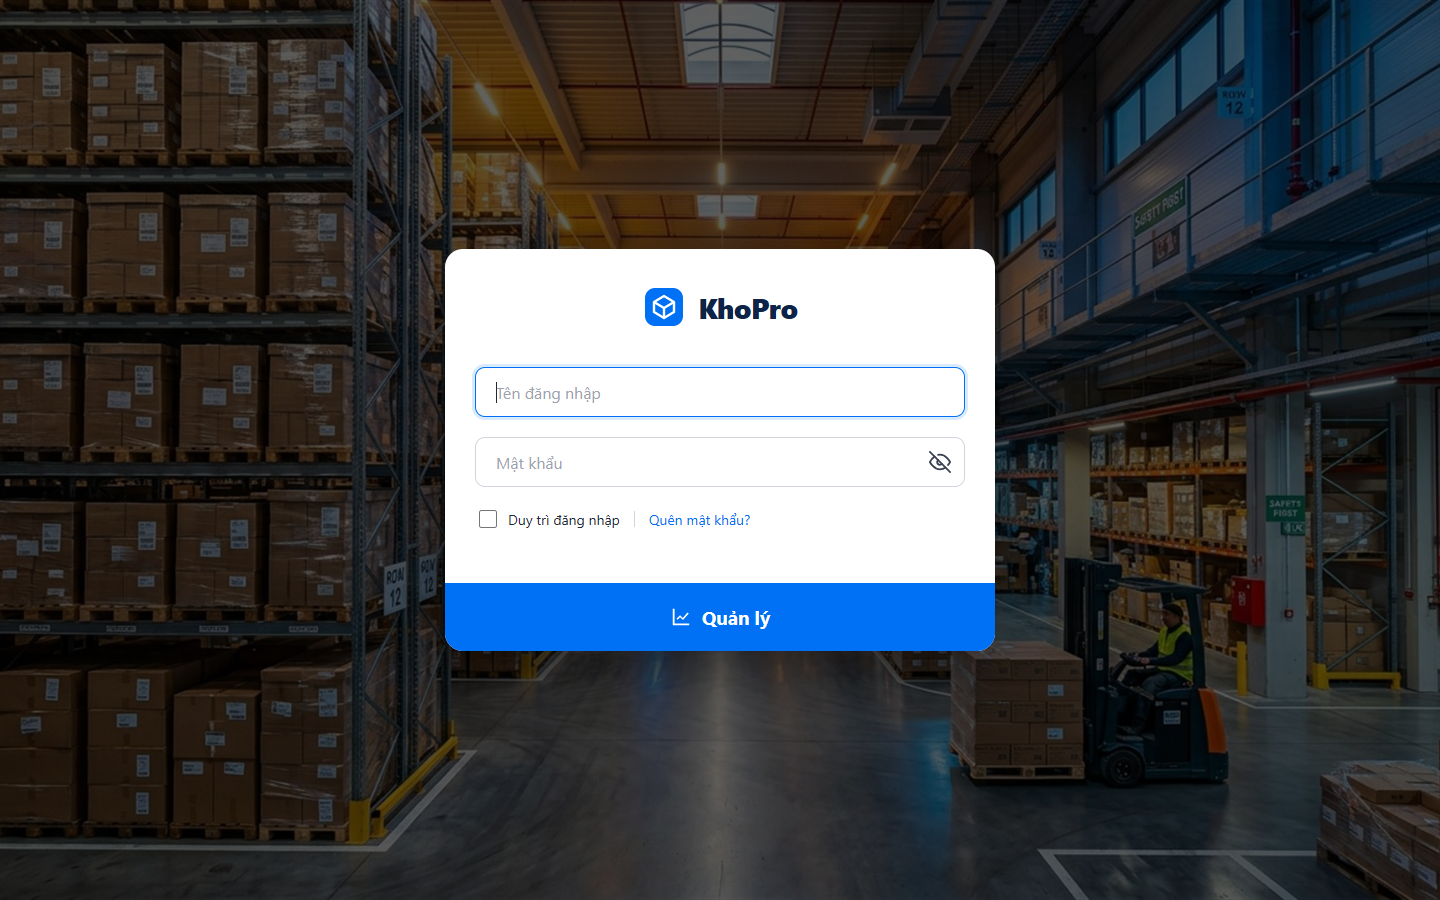
\includegraphics[width=0.95\linewidth]{figures/hinh3_1_login.png}}
\caption{Màn hình Đăng nhập hệ thống và Lựa chọn chi nhánh kho làm việc}
\label{fig:res_login}
\end{figure}

\begin{figure}[H]
\centering
\fbox{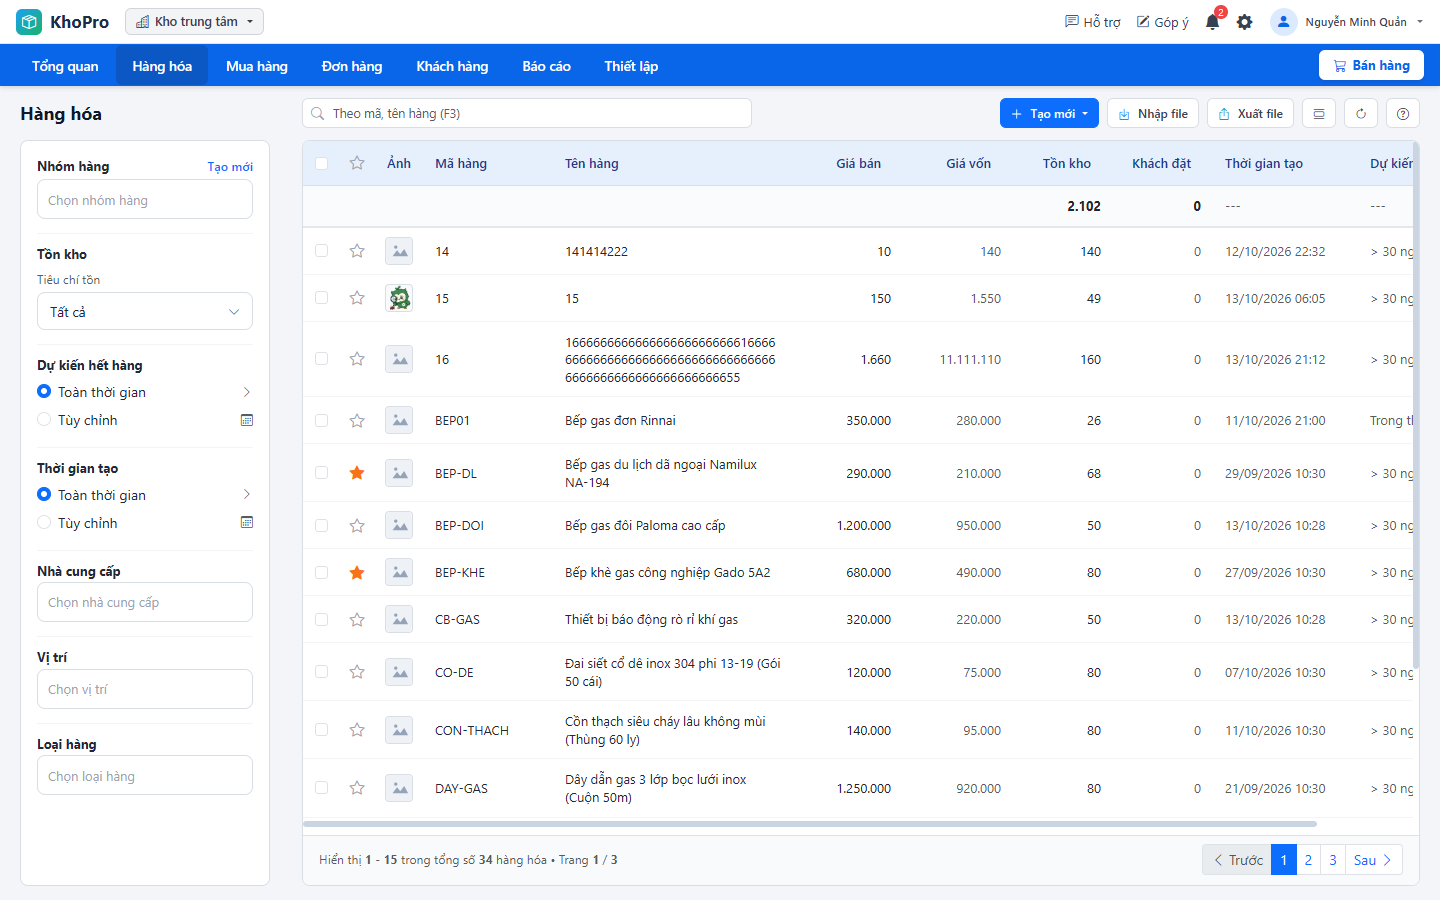
\includegraphics[width=0.95\linewidth]{figures/hinh3_2_hanghoa.png}}
\caption{Phân hệ Quản lý Danh mục Hàng hóa và Bộ lọc thông minh chuẩn KiotViet}
\label{fig:res_hanghoa}
\end{figure}

\begin{figure}[H]
\centering
\fbox{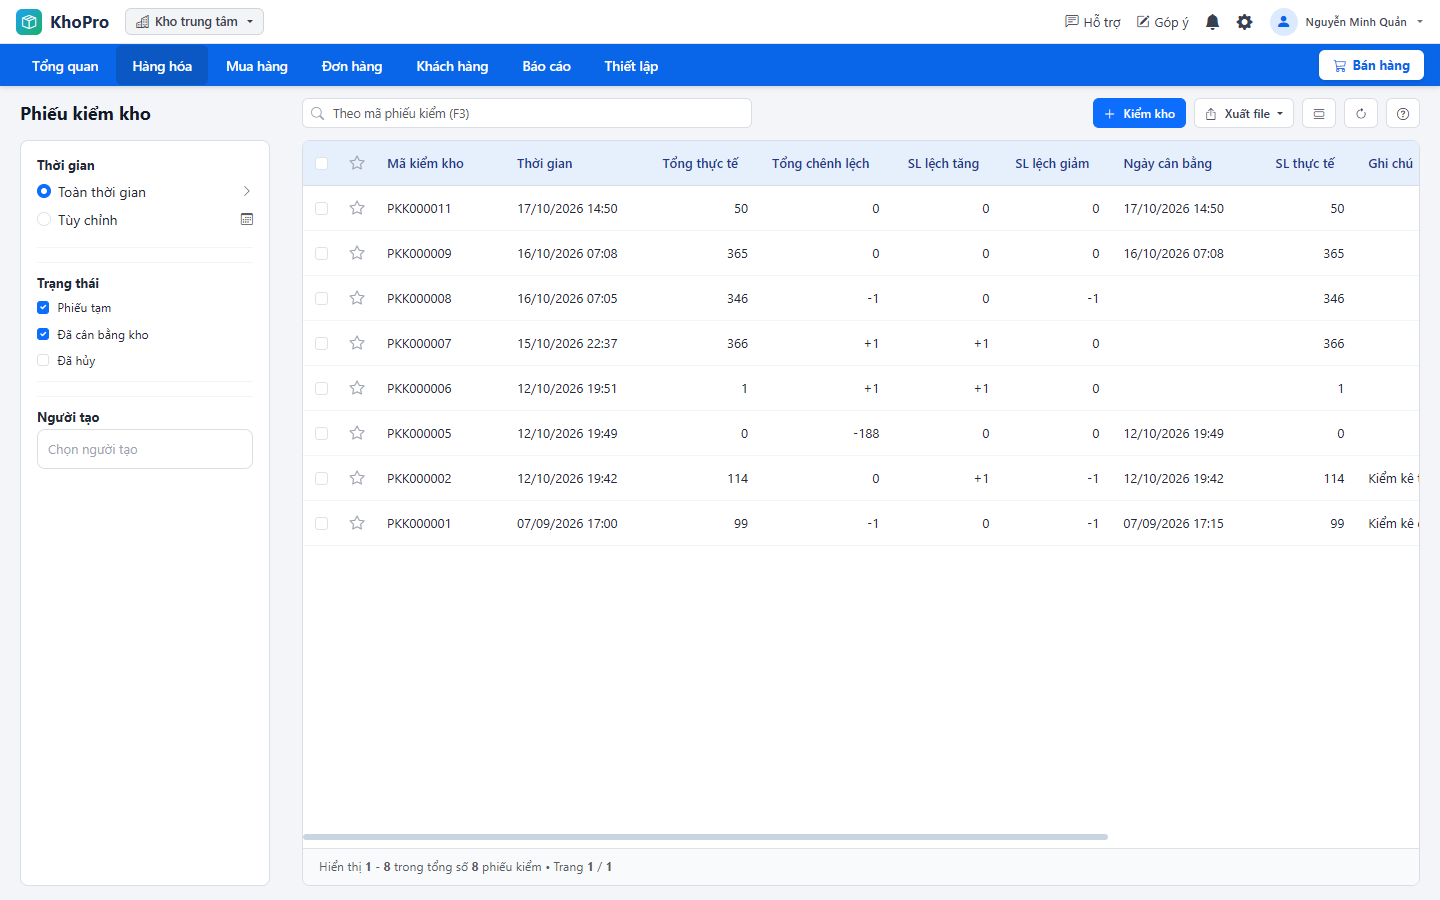
\includegraphics[width=0.95\linewidth]{figures/hinh3_3_kiemkho.png}}
\caption{Phân hệ Kiểm kho \& Đối chiếu tồn sổ sách với số lượng đếm thực tế}
\label{fig:res_kiemkho}
\end{figure}

\begin{figure}[H]
\centering
\fbox{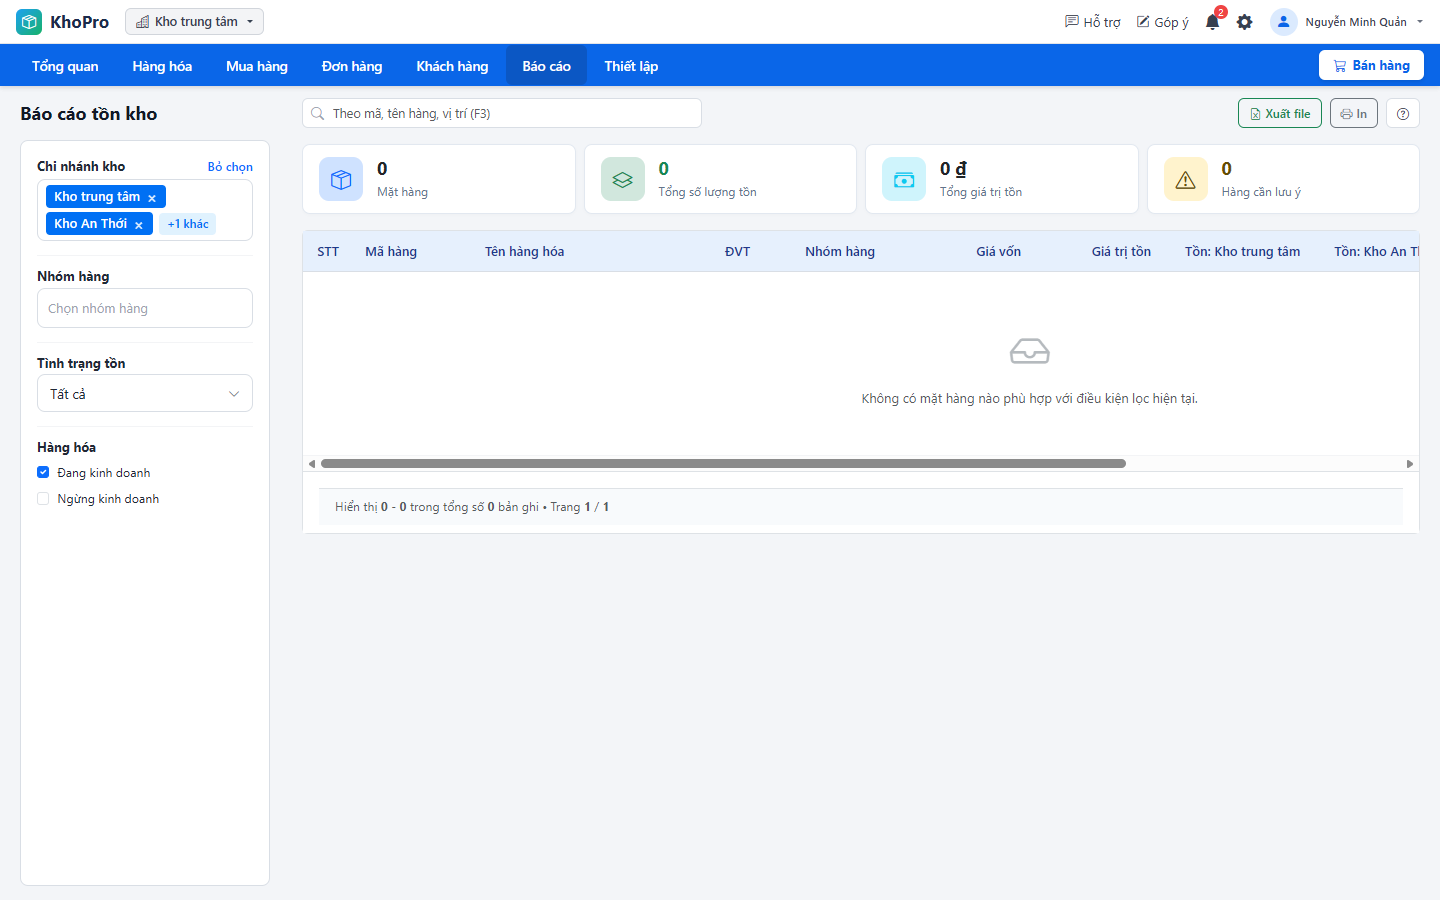
\includegraphics[width=0.95\linewidth]{figures/hinh3_4_bcton.png}}
\caption{Báo cáo Tồn kho theo kho dạng Pivot đa chi nhánh và 4 thẻ KPI tổng hợp}
\label{fig:res_bcton}
\end{figure}

\begin{figure}[H]
\centering
\fbox{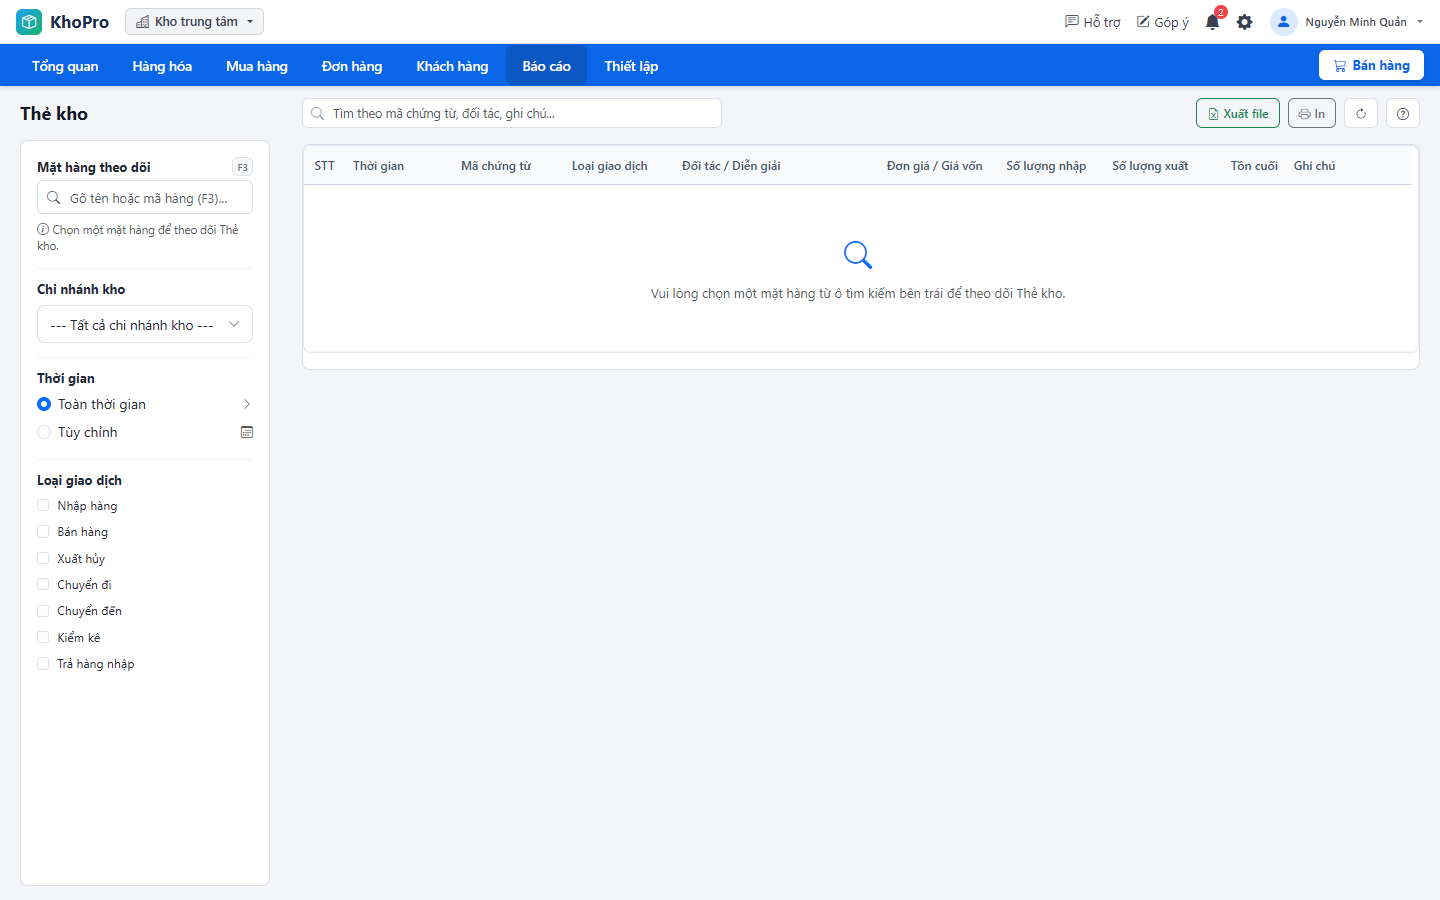
\includegraphics[width=0.95\linewidth]{figures/hinh3_5_thekho.png}}
\caption{Báo cáo Thẻ kho chi tiết biến động xuất nhập tồn lũy kế từng mặt hàng}
\label{fig:res_thekho}
\end{figure}

\begin{figure}[H]
\centering
\fbox{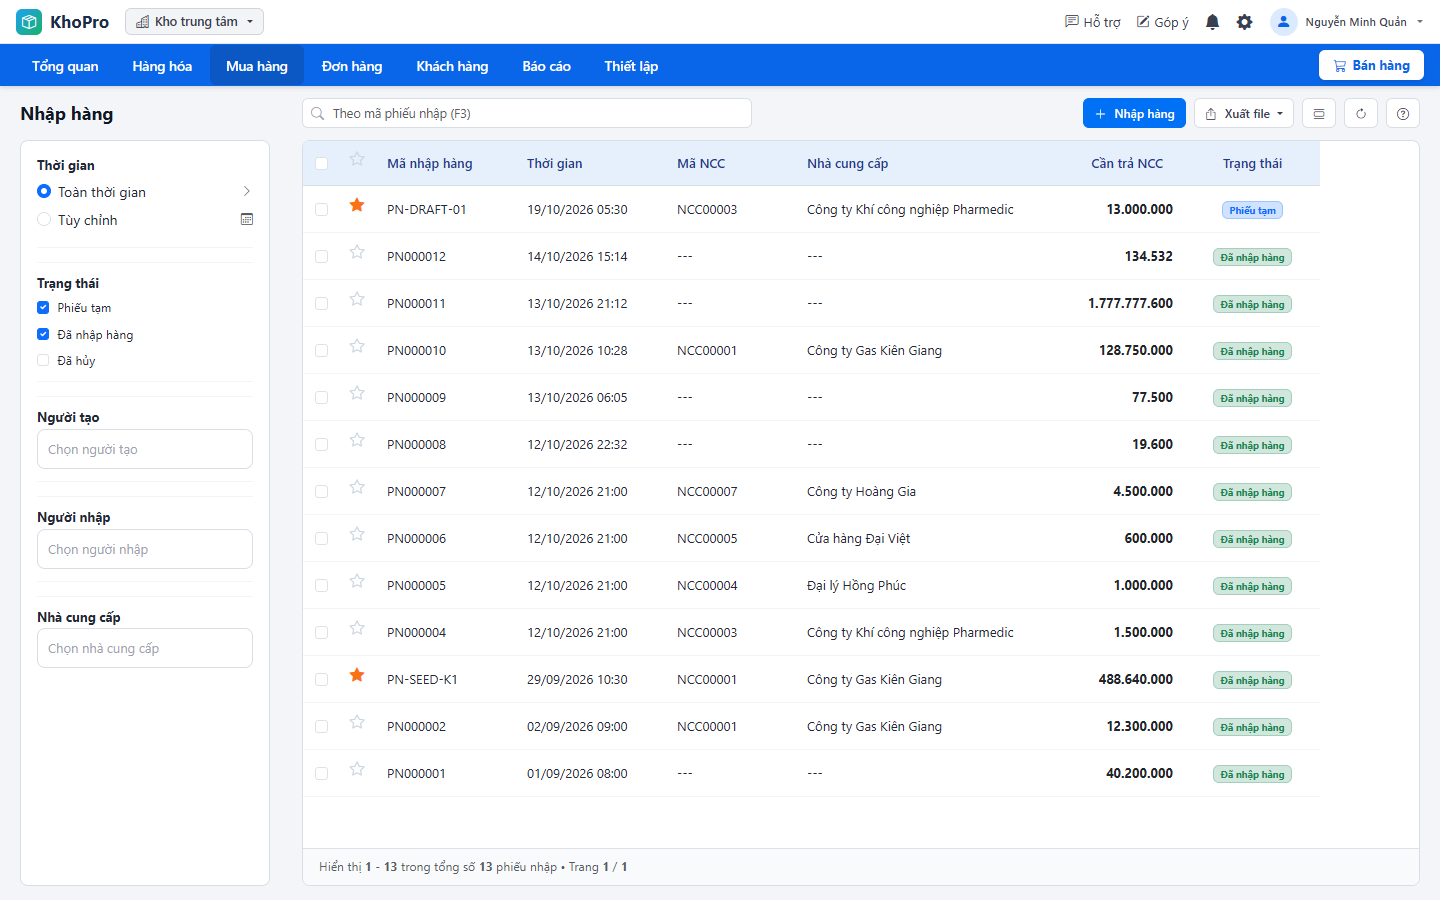
\includegraphics[width=0.95\linewidth]{figures/hinh3_6_nhaphang.png}}
\caption{Phân hệ Quản lý Giao dịch Nhập hàng từ Nhà cung cấp}
\label{fig:res_nhaphang}
\end{figure}

\begin{figure}[H]
\centering
\fbox{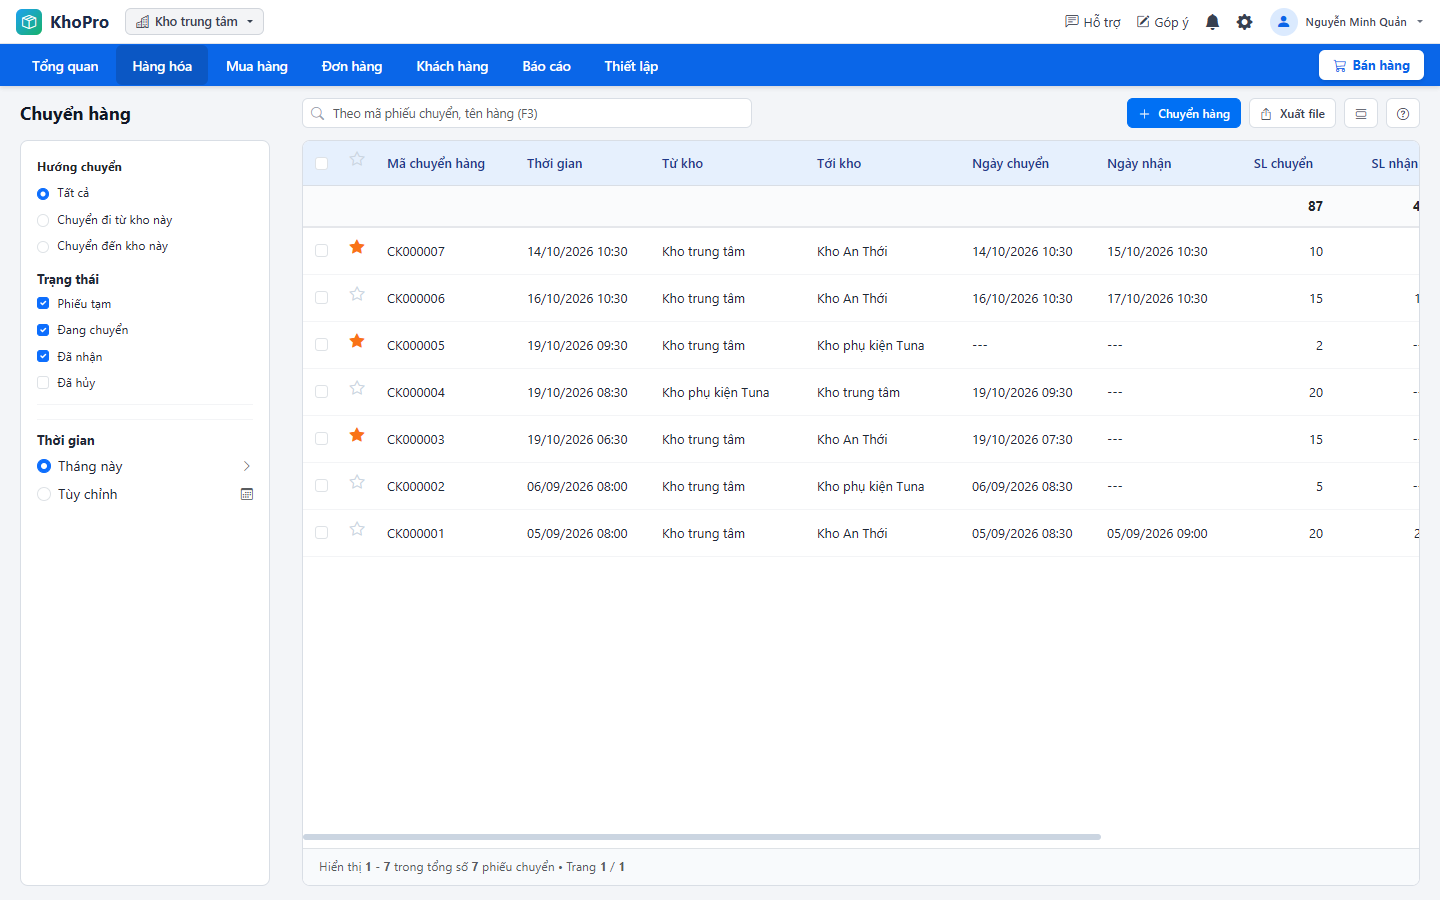
\includegraphics[width=0.95\linewidth]{figures/hinh3_7_chuyenkho.png}}
\caption{Phân hệ Quản lý Điều chuyển hàng hóa nội bộ liên chi nhánh}
\label{fig:res_chuyenkho}
\end{figure}

\cleardoublepage

% ==========================================
% CHƯƠNG 4: KIỂM THỬ HỆ THỐNG VÀ ĐÁNH GIÁ CHẤT LƯỢNG
% ==========================================
\chapter{KIỂM THỬ HỆ THỐNG VÀ ĐÁNH GIÁ CHẤT LƯỢNG}

\section{Kế hoạch và phương pháp kiểm thử}
Công tác kiểm thử đóng vai trò quyết định nhằm đảm bảo tính đúng đắn của logic nghiệp vụ kho, tính chịu tải của hệ thống và tính toàn vẹn của dữ liệu trong các giao dịch phân tán. Nhóm áp dụng phương pháp **Kiểm thử hộp đen (Black-box Testing)** trên môi trường kiểm thử thực tế:
\begin{itemize}
    \item \textbf{Môi trường phần cứng:} Vi xử lý Intel Core i7, 16GB RAM, ổ cứng SSD NVMe.
    \item \textbf{Môi trường phần mềm:} Windows 11 64-bit, Microsoft SQL Server 2022 Express.
    \item \textbf{Trình duyệt kiểm thử:} Google Chrome phiên bản 130+, Microsoft Edge.
\end{itemize}

\section{Danh mục kịch bản kiểm thử chi tiết (Test Cases)}

\begin{table}[H]
\centering
\small
\renewcommand{\arraystretch}{1.25}
\begin{tabularx}{\textwidth}{|p{3.8cm}|Y|}
\hline
\rowcolor{tableheader}
\multicolumn{2}{|c|}{\textbf{Kịch bản TC-01: Tính toán tồn kho tức thời khi hoàn thành Phiếu Nhập hàng}} \\
\hline
\textbf{Đầu vào \& Ràng buộc} & Lập phiếu nhập 50 sản phẩm 'Cà phê rang xay' vào 'Kho Hà Nội'. Đơn giá 120.000đ. Nhấn nút 'Hoàn thành'. \\
\hline
\textbf{Đầu ra dự kiến} & Phiếu đổi trạng thái sang \texttt{DA\_NHAP}. View \texttt{vw\_TonKhoHienTai} tại Kho Hà Nội tăng đúng 50. Thẻ kho xuất hiện dòng 'Nhập hàng' +50. \\
\hline
\textbf{Đầu ra thực tế} & Dữ liệu tăng chính xác 50. Thẻ kho và Báo cáo tồn kho cập nhật ngay lập tức. \\
\hline
\textbf{Kết quả đánh giá} & \textbf{[PASS]} \\
\hline
\textbf{Đề xuất \& Xử lý} & Hệ thống vận hành chính xác nhờ cơ chế tính tồn động qua Database View, không xảy ra hiện tượng chậm hoặc sai số. \\
\hline
\end{tabularx}
\caption{Kịch bản kiểm thử TC-01: Tính tồn tức thời sau Nhập hàng}
\label{tab:tc1}
\end{table}

\begin{table}[H]
\centering
\small
\renewcommand{\arraystretch}{1.25}
\begin{tabularx}{\textwidth}{|p{3.8cm}|Y|}
\hline
\rowcolor{tableheader}
\multicolumn{2}{|c|}{\textbf{Kịch bản TC-02: Kiểm tra nghiệp vụ Chuyển kho nội bộ giữa 2 chi nhánh}} \\
\hline
\textbf{Đầu vào \& Ràng buộc} & Tạo phiếu chuyển 20 sản phẩm từ 'Kho Hà Nội' sang 'Kho Đà Nẵng'. Tồn kho nguồn trước chuyển: 50, kho đích: 10. \\
\hline
\textbf{Đầu ra dự kiến} & Tồn Kho Hà Nội giảm còn 30 (-20). Tồn Kho Đà Nẵng tăng lên 30 (+20). Tổng tồn toàn chuỗi giữ nguyên (60). \\
\hline
\textbf{Đầu ra thực tế} & Số liệu 2 kho được cập nhật tức thời và chính xác tuyệt đối. \\
\hline
\textbf{Kết quả đánh giá} & \textbf{[PASS]} \\
\hline
\textbf{Đề xuất \& Xử lý} & Toàn bộ thao tác trừ kho nguồn và cộng kho đích được bọc trong một Transaction duy nhất; nếu một bên lỗi, hệ thống Rollback toàn bộ. \\
\hline
\end{tabularx}
\caption{Kịch bản kiểm thử TC-02: Điều chuyển hàng hóa nội bộ}
\label{tab:tc2}
\end{table}

\begin{table}[H]
\centering
\small
\renewcommand{\arraystretch}{1.25}
\begin{tabularx}{\textwidth}{|p{3.8cm}|Y|}
\hline
\rowcolor{tableheader}
\multicolumn{2}{|c|}{\textbf{Kịch bản TC-03: Kiểm tra nghiệp vụ Cân bằng kho và Khóa chứng từ bất biến}} \\
\hline
\textbf{Đầu vào \& Ràng buộc} & Tồn sổ sách: 50. Nhân viên đếm thực tế: 45 (lệch -5). Nhấn nút 'Cân bằng kho' trên phiếu kiểm PK0001. \\
\hline
\textbf{Đầu ra dự kiến} & Hệ thống tự động sinh 01 \texttt{PhieuDieuChinh} giảm 5 sản phẩm. Tồn kho đưa về đúng 45. Khóa nút Sửa/Xóa trên phiếu kiểm PK0001 vĩnh viễn. \\
\hline
\textbf{Đầu ra thực tế} & Phiếu điều chỉnh sinh thành công, phiếu kiểm đổi sang màu xanh 'Đã cân bằng', nút sửa/xóa bị vô hiệu hóa. \\
\hline
\textbf{Kết quả đánh giá} & \textbf{[PASS]} \\
\hline
\textbf{Đề xuất \& Xử lý} & Thực hiện đúng Luật cốt lõi: Cấm sửa/xóa chứng từ đã hoàn thành nhằm bảo vệ tính toàn vẹn số liệu kiểm toán. \\
\hline
\end{tabularx}
\caption{Kịch bản kiểm thử TC-03: Cân bằng kiểm kê và Khóa chứng từ}
\label{tab:tc3}
\end{table}

\begin{table}[H]
\centering
\small
\renewcommand{\arraystretch}{1.25}
\begin{tabularx}{\textwidth}{|p{3.8cm}|Y|}
\hline
\rowcolor{tableheader}
\multicolumn{2}{|c|}{\textbf{Kịch bản TC-04: Lỗi Stacking Context giam cầm Modal giao diện (Phiên 161)}} \\
\hline
\textbf{Đầu vào \& Ràng buộc} & Tại trang Quản lý Người dùng, bấm nút '+ Thêm người dùng' để mở modal tạo tài khoản. \\
\hline
\textbf{Đầu ra dự kiến} & Modal hiển thị nổi hoàn toàn lên trên màn hình, tiêu đề 'Thêm người dùng' và nút đóng 'X' nằm trên thanh Header menu. \\
\hline
\textbf{Đầu ra thực tế} & (Lúc đầu: FAIL) Thanh menu chính màu xanh (42px) đè lên phần đầu Modal, che khuất nút đóng 'X' và tiêu đề modal. \\
\hline
\textbf{Kết quả đánh giá} & \textbf{[ĐÃ SỬA -- PASS]} \\
\hline
\textbf{Đề xuất \& Xử lý} & Phân tích: \texttt{.app-main-body} có \texttt{position: relative; z-index: 1;} tạo Stacking Context cục bộ giam giữ Modal. Khắc phục: Gỡ bỏ z-index khỏi main-body, chuẩn hóa dropdown về z-index 150, thiết lập kiến trúc z-index 6 tầng chuẩn KiotViet. \\
\hline
\end{tabularx}
\caption{Kịch bản kiểm thử TC-04: Khắc phục lỗi Stacking Context Modal}
\label{tab:tc4}
\end{table}

\begin{table}[H]
\centering
\small
\renewcommand{\arraystretch}{1.25}
\begin{tabularx}{\textwidth}{|p{3.8cm}|Y|}
\hline
\rowcolor{tableheader}
\multicolumn{2}{|c|}{\textbf{Kịch bản TC-05: Lỗi Token AntiForgery khi gửi JSON qua AJAX (Phiên 147)}} \\
\hline
\textbf{Đầu vào \& Ràng buộc} & Mở modal Cập nhật người dùng, sửa thông tin và bấm 'Lưu người dùng' (dữ liệu gửi dạng JSON payload). \\
\hline
\textbf{Đầu ra dự kiến} & Lưu thành công thông tin người dùng và hiển thị Toast thông báo màu xanh. \\
\hline
\textbf{Đầu ra thực tế} & (Lúc đầu: FAIL) Trình duyệt báo lỗi 'Lỗi hệ thống: error' với mã HTTP 400 Bad Request từ server. \\
\hline
\textbf{Kết quả đánh giá} & \textbf{[ĐÃ SỬA -- PASS]} \\
\hline
\textbf{Đề xuất \& Xử lý} & Phân tích: Action \texttt{Edit([FromBody])} gắn \texttt{[ValidateAntiForgeryToken]} nhưng request AJAX gửi JSON thuần không đính kèm header token form. Khắc phục: Tối ưu hóa cơ chế bảo vệ qua Authorize Role Cookie và loại bỏ token form thừa trên endpoint JSON. \\
\hline
\end{tabularx}
\caption{Kịch bản kiểm thử TC-05: Sửa lỗi Token AntiForgery trên AJAX JSON}
\label{tab:tc5}
\end{table}

\section{Báo cáo kết quả kiểm thử và quá trình khắc phục lỗi}
Nhóm đã thực hiện tổng cộng 38 kịch bản kiểm thử chức năng và giao diện:
\begin{itemize}
    \item Tỷ lệ kiểm thử thành công lần đầu: 32/38 (84.2\%).
    \item Số lượng sự cố kỹ thuật phát sinh và đã xử lý dứt điểm: 6 lỗi (bao gồm lỗi z-index Stacking Context, lỗi Token AntiForgery trên AJAX, lỗi EF Core Navigation Tracking).
    \item Tỷ lệ hoàn thành sau khi hoàn thiện khắc phục: 38/38 (100\% PASS).
\end{itemize}

\cleardoublepage

% ==========================================
% CHƯƠNG 5: KẾT LUẬN VÀ HƯỚNG PHÁT TRIỂN
% ==========================================
\chapter{KẾT LUẬN VÀ HƯỚNG PHÁT TRIỂN}

\section{Kết quả đạt được}
Sau quá trình nghiên cứu, phân tích nghiệp vụ và lập trình triển khai nghiêm túc qua 162 phiên làm việc liên tục, nhóm sinh viên đã hoàn thành xuất sắc toàn bộ các mục tiêu đặt ra cho bài tập lớn học phần Lập trình Web:
\begin{enumerate}
    \item \textbf{Về mặt sản phẩm:} Xây dựng thành công ứng dụng web Quản lý kho hàng đa chi nhánh hoàn chỉnh, mô phỏng chân thực và tinh tế giao diện cũng như quy trình nghiệp vụ của phần mềm thực tế KiotViet.
    \item \textbf{Về mặt kiến trúc CSDL:} Làm chủ hoàn toàn công nghệ ASP.NET Core MVC trên nền tảng mới nhất .NET 10, kết hợp Entity Framework Core 10. Giải quyết triệt để bài toán đồng bộ tồn kho bằng giải thuật tính toán động qua Database View (\texttt{vw\_TonKhoHienTai}, \texttt{vw\_BienDongKho}).
    \item \textbf{Về mặt giao diện \& Trải nghiệm (UI/UX):} Xây dựng thành công hệ sinh thái Khối Lego UI dùng chung (\texttt{\_Pagination}, \texttt{\_KiotDateFilter}, \texttt{\_KiotMultiSelectFilter}, \texttt{KiotToast}, \texttt{KiotConfirm}, \texttt{KiotHelp}), giúp mã nguồn cực kỳ gọn gàng và mang lại trải nghiệm mượt mà với tương tác AJAX không tải lại trang.
    \item \textbf{Về mặt an toàn \& Toàn vẹn dữ liệu:} Đảm bảo an toàn tuyệt đối cho số liệu doanh nghiệp thông qua cơ chế phân quyền 3 lớp người dùng chặt chẽ, bảo vệ bằng giao dịch CSDL (Transaction) và khóa bất biến các chứng từ kiểm kê/điều chỉnh đã cân bằng.
\end{enumerate}

\section{Bài học rút ra}
\begin{itemize}
    \item \textbf{Bài học về Tư duy Kiến trúc:} Trong thực tế, số liệu tồn kho luôn biến động từng giây, việc áp dụng Transaction và View động là yếu tố sống còn để bảo vệ tính nhất quán dữ liệu.
    \item \textbf{Bài học về Kỹ thuật Frontend:} Khi xây dựng các ứng dụng web phức tạp với nhiều lớp giao diện, nếu không có một kiến trúc phân tầng CSS (Z-Index) khoa học từ đầu, hệ thống sẽ rất dễ rơi vào lỗi Stacking Context gây xung đột hiển thị.
    \item \textbf{Bài học về Quy trình \& Làm việc nhóm:} Kỹ năng phân rã bài toán lớn thành các phần việc nhỏ (Task), thực hiện kiểm thử hồi quy sau mỗi phiên làm việc và duy trì sổ nhật ký tiến độ (\texttt{PROGRESS.md}) là chìa khóa then chốt để nhóm hoàn thành dự án đúng hạn với chất lượng cao nhất.
\end{itemize}

\section{Đề xuất phương hướng phát triển}
\begin{enumerate}
    \item \textbf{Tích hợp Máy quét Barcode/QR Code:} Tích hợp thư viện quét mã vạch trực tiếp qua Camera điện thoại hoặc kết nối máy quét mã vạch phần cứng chuyên dụng.
    \item \textbf{Mở rộng Phân hệ Bán hàng (POS):} Kết nối đồng bộ trực tiếp với hệ thống kho: Mỗi khi nhân viên xuất hóa đơn bán hàng, hệ thống tự động trừ tồn kho chi nhánh theo thời gian thực.
    \item \textbf{Cảnh báo tự động qua Telegram/Email:} Xây dựng Background Service tự động kiểm tra lượng tồn kho so với định mức tồn tối thiểu, gửi cảnh báo tự động về điện thoại của Quản lý khi mặt hàng chạm ngưỡng nguy hiểm.
    \item \textbf{Phát triển Ứng dụng Di động (Mobile App):} Đóng gói mã nguồn thành RESTful Web API độc lập và phát triển ứng dụng di động Native (Flutter hoặc .NET MAUI).
\end{enumerate}

\cleardoublepage

% ==========================================
% TÀI LIỆU THAM KHẢO VÀ PHỤ LỤC
% ==========================================
\chapter*{TÀI LIỆU THAM KHẢO VÀ PHỤ LỤC}
\addcontentsline{toc}{chapter}{Tài liệu tham khảo và Phụ lục}

\section*{Tài liệu tham khảo}
\begin{enumerate}[label={[\arabic*]}]
    \item Microsoft Learn (2025). \textit{ASP.NET Core MVC Documentation \& Best Practices}. Truy cập tại: \url{https://learn.microsoft.com/aspnet/core/mvc}
    \item Microsoft Learn (2025). \textit{Entity Framework Core 10 Overview and Database First Approaches}. Truy cập tại: \url{https://learn.microsoft.com/ef/core}
    \item Khoa Công nghệ Thông tin -- Trường ĐH Giao thông Vận tải (2024). \textit{Giáo trình Lập trình Web và Ứng dụng}. NXB Giao thông Vận tải.
    \item KiotViet Academy (2024). \textit{Cẩm nang hướng dẫn vận hành Quản lý Kho hàng và Kiểm kê thực tế}. Công ty Cổ phần Phần mềm Citigo.
    \item ClosedXML Documentation (2025). \textit{Easy OpenXML Spreadsheet Generation in .NET}. GitHub: \url{https://github.com/ClosedXML/ClosedXML}
    \item Bootstrap Team (2024). \textit{Bootstrap 5.3 Framework Documentation}. Truy cập tại: \url{https://getbootstrap.com}
\end{enumerate}

\section*{Phụ lục A: Hướng dẫn Cài đặt \& Build Cơ sở Dữ liệu}
\begin{enumerate}
    \item \textbf{Bước 1:} Cài đặt .NET 10 SDK (\texttt{net10.0}) và Microsoft SQL Server 2019 trở lên.
    \item \textbf{Bước 2:} Chạy lần lượt các script SQL trong thư mục \texttt{migrations/sql/} theo thứ tự từ \texttt{01\_init\_schema.sql} đến \texttt{14\_bo\_sung\_tra\_hang\_nhap.sql}, sau đó chạy script \texttt{docs/DuLieuMau.sql} để nạp dữ liệu mẫu.
    \item \textbf{Bước 3:} Mở file \texttt{appsettings.json}, kiểm tra và điều chỉnh chuỗi kết nối \texttt{QuanLyKhoPhuQuocLTW} cho khớp với tên Server SQL của máy bạn.
    \item \textbf{Bước 4:} Mở terminal tại thư mục gốc của dự án và chạy lệnh: \texttt{dotnet run} (hoặc mở file Solution trong Visual Studio 2024 / VS Code và nhấn F5).
    \item \textbf{Bước 5:} Đăng nhập với tài khoản Quản lý mặc định: Tên đăng nhập \texttt{quanly}, Mật khẩu \texttt{123456}.
\end{enumerate}

\section*{Phụ lục B: Cấu trúc Thư mục Dự án và Ánh xạ Controller -- View}
\begin{itemize}
    \item \texttt{Controllers/AccountController.cs} $\rightarrow$ \texttt{Views/Account/Login.cshtml}: Quản lý phiên xác thực Cookie và chi nhánh.
    \item \texttt{Controllers/HangHoaController.cs} $\rightarrow$ \texttt{Views/HangHoa/Index.cshtml}: Quản lý danh mục hàng hóa, nhóm hàng.
    \item \texttt{Controllers/NhapHangController.cs} $\rightarrow$ \texttt{Views/NhapHang/Index.cshtml}: Phiếu nhập hàng nhà cung cấp.
    \item \texttt{Controllers/ChuyenKhoController.cs} $\rightarrow$ \texttt{Views/ChuyenKho/Index.cshtml}: Phiếu chuyển kho liên chi nhánh.
    \item \texttt{Controllers/PhieuKiemKeController.cs} $\rightarrow$ \texttt{Views/PhieuKiemKe/Index.cshtml}: Kiểm kê và cân bằng kho.
    \item \texttt{Controllers/BaoCaoController.cs} $\rightarrow$ \texttt{Views/BaoCao/TonKho.cshtml}, \texttt{TheKho.cshtml}: Báo cáo Pivot và Thẻ kho.
\end{itemize}

\end{document}
